\documentclass[notes]{beamer}           % print frame + notes
% \documentclass[notes=only]{beamer}    % only notes
% \documentclass{beamer}                % only frames

\usepackage[utf8]{inputenc}
\usepackage{amsmath}
\usepackage{amsthm}
\usepackage{mathtools}
\usepackage{algorithmic,float}
\usepackage[linesnumbered, ruled]{algorithm2e}
\usepackage{graphicx}
\usepackage{media9}

% Adds do-while syntax for algorithms
\SetKwRepeat{Do}{do}{while}%

% Case Statements for Proofs
\newcounter{case}[section]
\newenvironment{case}[1][]{\refstepcounter{case}\par\medskip
   \textbf{Case~\thecase. #1} \rmfamily}{\medskip}
   
\newcounter{subcase}[case]
\newenvironment{subcase}[1][]{\refstepcounter{subcase}\par\medskip
   \textbf{Case~\thecase.\thesubcase. #1} \rmfamily}{\medskip}

% Give names to lemmas
\newtheoremstyle{named}{}{}{\itshape}{}{\bfseries}{.}{.5em}{\thmnote{#3's }#1}
\theoremstyle{named}
\newtheorem*{namedlemma}{Lemma}

% Multi-part proofs
\makeatletter
\newenvironment<>{proofs}[1][\proofname]{%
    \par
    \def\insertproofname{#1\@addpunct{.}}%
    \usebeamertemplate{proof begin}#2}
  {\usebeamertemplate{proof end}}
\makeatother

% Section Title Slides
\AtBeginSection[]{
  \begin{frame}
  \vfill
  \centering
  \begin{beamercolorbox}[sep=8pt,center,shadow=true,rounded=true]{title}
    \usebeamerfont{title}\insertsectionhead\par%
  \end{beamercolorbox}
  \vfill
  \end{frame}
}

% Title Stuff
\title{Optimal Pattern Formation for Systems of Mobile Robots}
\author{Jared Coleman}
\institute{California State University, Long Beach}
\date{December 10, 2019}

% Changes multi-slide frame numbering to "Cont."
\setbeamertemplate{frametitle continuation}[from second][(Cont.)]

% Slides
\begin{document}
    \frame{\titlepage}

    \begin{frame}{Introduction}
        \framesubtitle{Motivation}

        Teams of robots often need to form Patterns for exploration, communication, etc.

        The size and orientation of the pattern may not matter, but each robot must conserve energy.
    \end{frame}

    \begin{frame}{Introduction}
        \framesubtitle{The Problem}
        
        \begin{columns}
            \begin{column}{0.5\textwidth}
                \begin{itemize}
                    \item A set of robots with initially arbitrary positions must move to form a pattern.
                    \item Patterns are invariant to translation, rotation, and uniform scaling.
                \end{itemize}
            \end{column}
            \begin{column}{0.5\textwidth}
                \begin{center}
                    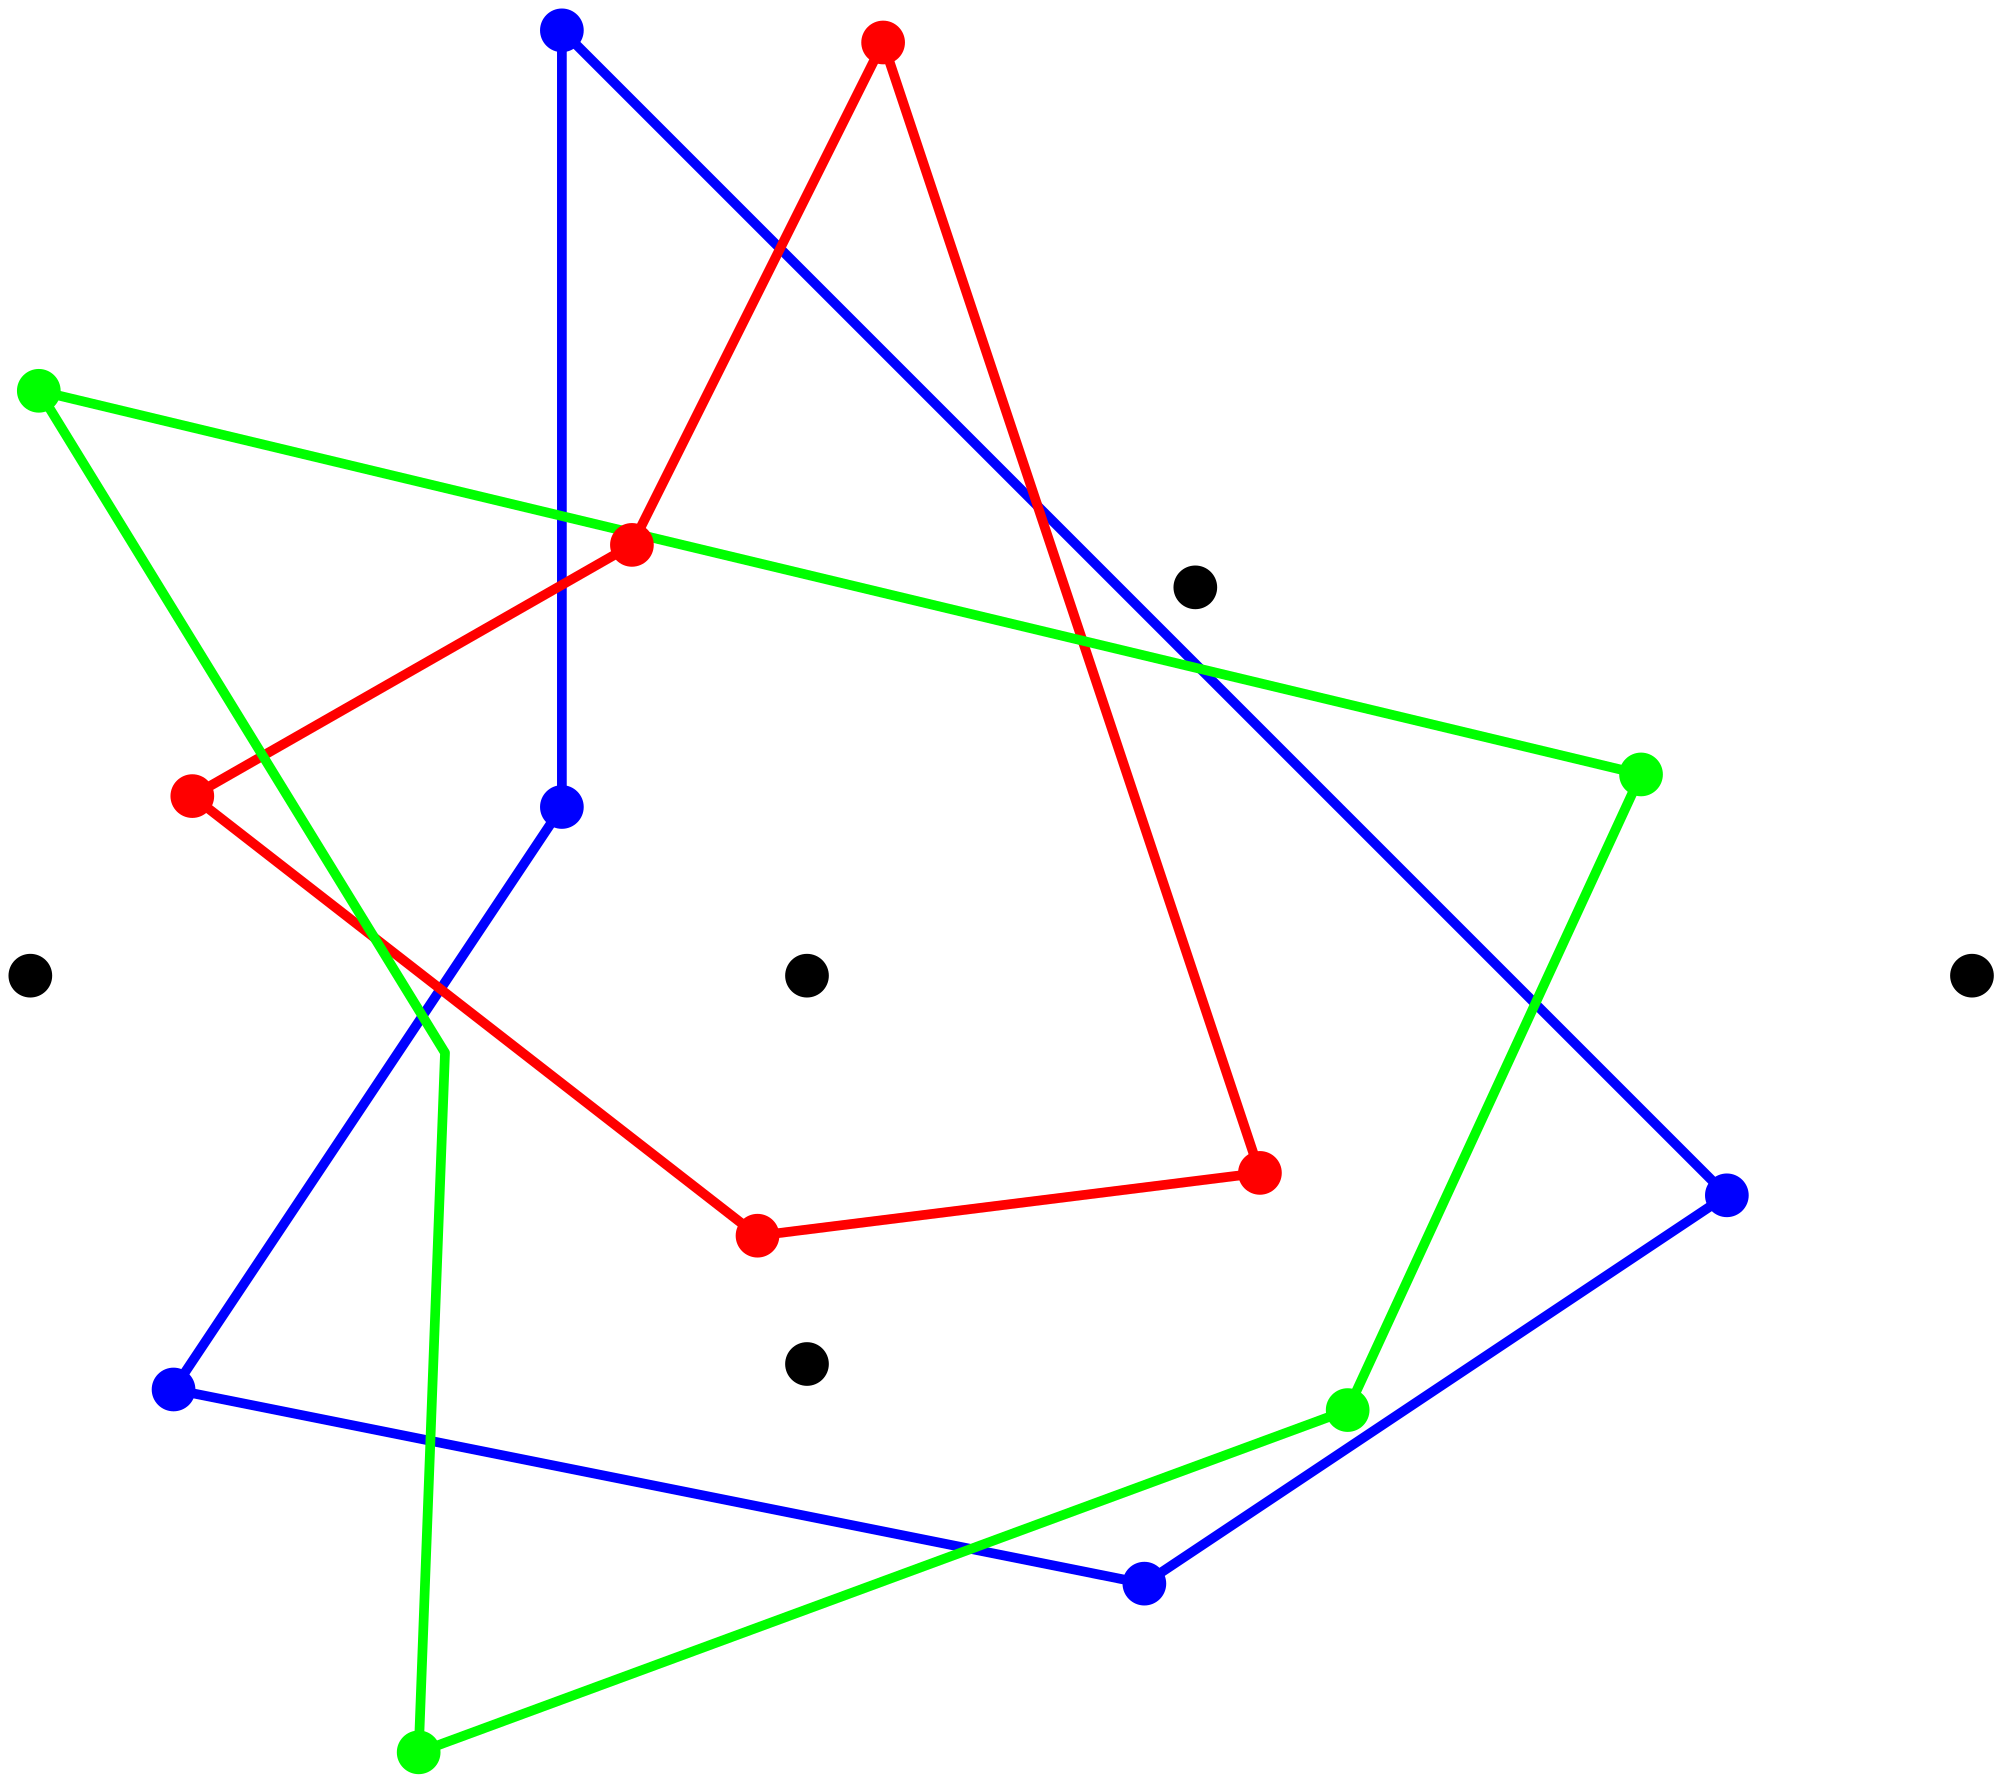
\includegraphics[width=\textwidth]{../media/intro_formations.png}
                \end{center}
            \end{column}
        \end{columns}
    \end{frame}

    \begin{frame}{Model \& Assumptions}
        \begin{itemize}
            \item Robots follow the \textit{Look}, \textit{Compute}, \textit{Move} model
            \begin{itemize}
                \item \textit{Look}: Robots observe the positions of all other robots.
                \item \textit{Compute}: Robots compute their destination in the optimal formation
                \item \textit{Move}: Robots move toward their destination
            \end{itemize}
            \item All robots execute the \textit{LCM} cycle synchronously
            \item Robots move at the same speed
        \end{itemize}
    \end{frame}

    \begin{frame}{Preliminaries}
        \begin{itemize}
            \item Calligraphic notation (e.g. $\mathcal{S}$, $\mathcal{M}$) for sets of sets of points.
            \item Capital letters for sets of points (e.g. $S$, $M$)
            \begin{itemize}
                \item $S^i$ is the $i^{th}$ point in $\mathcal{S}$
            \end{itemize}
            \item lower-case letters for points (e.g. $s$, $m$)
            \begin{itemize}
                \item $s^i_j$ is the $j^{th}$ point in $S^i$
            \end{itemize}
            \item $d(p, q)$ is the euclidian distance between points $p$ and $q$.
            \item $C(p, r)$ is a circle centered at $p$ with radius $r$.
            \item $D(p, r)$ is the closed disk centered at $p$ with radius $r$.
        \end{itemize}
    \end{frame}

    \begin{frame}
        \frametitle{Problem}

        Given two sets of points, $P$ and $S$ that represent the robots' original positions and a desired pattern, respectively, find the minimum maximum distance traveled by any robot necessary to form $S$:

        \begin{align*}
            d^* = \underset{Q \sim S}{min} ~ \underset{0 \leq i < n}{max} \sim d(p_i, q_i)
        \end{align*}

        Let $Q^*$ be the formation that yields the optimal solution $d^*$.
    \end{frame}

    \begin{frame}[allowframebreaks]{Necessary Conditions}
        \framesubtitle{Minimum Rigidness}
        \begin{lemma}
            For any set of points $P$ with optimal solution $d^*$, at least three robots move exactly $d^*$.
        \end{lemma}

        \framebreak

        \begin{columns}
            \begin{column}{0.6\textwidth}
                \begin{proofs}
                    \begin{case}
                        Suppose exactly $1$ robot, $r_0$, moves distance $d^*$ and all others move some distance less than or equal to $d^\prime < d^*$.
        
                        \bigskip
            
                        We can achieve a better solution by translating $Q^*$ some arbitrarily small $\epsilon < d^\prime$ so that $d(q_0, p_0) = d^* - \epsilon$ and $d(q_i, p_i) \leq d^\prime + \epsilon < d^*$ for $i \neq 0$.
        
                        \bigskip
                        
                        This is contradictory to $Q^*$ being optimal.
                    \end{case}
                \end{proofs}
            \end{column}
            \begin{column}{0.4\textwidth}
                \begin{center}
                    \includegraphics[width=\textwidth]{../media/onerobots.pdf}
                \end{center}
            \end{column}
        \end{columns}

        \framebreak
        
        \begin{columns}
            \begin{column}{0.6\textwidth}
                \begin{proof}[\proofname\ (Cont.)]
                    \begin{case}
                        Now suppose exactly $2$ robots, $r_0$ and $r_1$, move distance $d^*$ and all other robots move some distance less than or equal to $d^\prime < d^*$.
        
                        \bigskip
            
                        We can achieve a better solution by scaling and rotating $Q^*$ around $q_0$ some arbitrarily small amount such that $d(q_0, p_0) = d^* - \epsilon$ and $d(q_i, p_i) \leq d^\prime + \epsilon_i < d^*$ for $2 \leq i < n$. 
        
                        \bigskip
        
                        This reduces to Case 1.
                    \end{case}
                \end{proof}
            \end{column}
            \begin{column}{0.4\textwidth}
                \begin{center}
                    \includegraphics[width=\textwidth]{../media/tworobots.pdf}
                \end{center}
            \end{column}
        \end{columns}
        
    \end{frame}

    \begin{frame}[allowframebreaks]{A Motivating Example}
        Three robots need to form an equilateral triangle. 
        \bigskip

        Suppose we have access to an Oracle that, given a distance $r$, gives us a set of equidistant points $Q$ such that $d(q_i, p_i) = r$, if one exists.

        \framebreak

        A Reasonable solution would be to use a modified binary search:

        \begin{algorithm}[H]
            \algsetup{linenosize=\tiny}
            \SetKwFunction{FApproximateOptimalSolution}{ApproximateOptimalSolution}
            \SetKwProg{Fn}{Function}{:}{}

            \Fn{\FApproximateOptimalSolution{$P$, $\epsilon$}}{
                $low \gets 0$\;
                $high \gets \underset{i,j \in [0, |P|)}{max} d(r_i, r_j)$\;
                \Do{$high-low > 2\epsilon$} {
                    $r \gets \frac{high-low}{2}$\;
                    $Q \gets Oracle(r)$\;
                    \eIf{$Q$ is null}{
                        $low = r$\;
                    }{
                        $high = r$\;
                    }
                } 
                \Return $Q$\;
            }
        \end{algorithm}
        
        \framebreak

        \begin{itemize}
            \item \texttt{ApproximateOptimalSolution} runs in 
            $\mathcal{O}\left(log\left(\frac{d}{\epsilon}\right)\right)$ 
            where $d$ is the greatest distance between any two robots and $\epsilon$ is the acceptable error for the solution.
            \item \texttt{ApproximateOptimalSolution} is an \textit{approximation} - \textbf{not optimal}.
            \item Each robot is guaranteed to move no more than $\epsilon$ further than in the optimal solution.
            \item \textbf{Spoiler}: We propose a fixed-step, ruler-and-compass method for computing the optimal solution
        \end{itemize}
    \end{frame}

    \section{Three Robots}

    \begin{frame}[allowframebreaks]{Replication}
        \begin{itemize}
            \item A tool we based on pure geometry that resembles a pantograph.
            \item Used to derive later results.
        \end{itemize}

        \framebreak
        
        \begin{definition}[Trivial Replication]
            The Trivial Replication, $R_{Trivial}(P, q_0, q_1)$, is the set of points similar to $P$ whose first and second point are $q_0$ and $q_1$, respectively.
        \end{definition}

        \framebreak

        \begin{columns}
            \begin{column}{0.7\textwidth}
                \begin{definition}[Replication Machine]
                    The Replication Machine, $R_{Machine}(P, q_0, q_1, r)$, is the infinite set of shapes similar to $P$ whose first point is $q_0$ and second point is on the circumference of the circle centered at $q_1$ with radius $r$.                     
                \end{definition}
            \end{column}
            \begin{column}{0.3\textwidth}
                \begin{center}
                    \includemedia[
                        width=0.75\textwidth,height=0.75\linewidth,
                        activate=pageopen,
                        transparent,
                        addresource=../media/replication_machine.mp4,
                        flashvars={source=../media/replication_machine.mp4&autoPlay=true&loop=true}
                      ]{}{VPlayer.swf}
                \end{center}
            \end{column}
        \end{columns}

        \framebreak

        \begin{columns}
            \begin{column}{0.7\textwidth}
                \begin{definition}[Replication Spanner]
                    The Replication Spanner, $R_{Span}(P, q_0, q_1, r)$, is the infinite set of shapes similar to $P$ whose first and second points are on the circumferences of the circles with radius $r$ centered at $q_0$ and $q_1$, respectively.                 
                \end{definition}
            \end{column}
            \begin{column}{0.3\textwidth}
                \begin{center}
                    \includemedia[
                        width=0.75\textwidth,height=0.75\linewidth,
                        activate=pageopen,
                        transparent,
                        addresource=../media/replication_spanner.mp4,
                        flashvars={source=../media/replication_spanner.mp4&autoPlay=true&loop=true}
                      ]{}{VPlayer.swf}
                \end{center}
            \end{column}
        \end{columns}

    \end{frame}

    \note{
        Add picture of pantograph (and a little history)
    }

    \begin{frame}[allowframebreaks]{Replication Machine Circles}

        Given a formation $P$ of size $n$, points $q_0$ and $q_1$, and a distance $r$.

        \begin{lemma}
            The $n$ sets of $i^{th}$ points in the replicated shapes each form a circle centered at $t_i$ with radius 
            $r\frac{d(q_0, t_i)}{d(q_0, q_1)}$.
        \end{lemma}

        \framebreak

        \begin{columns}
            \begin{column}{0.5\textwidth}       
                \begin{proofs}
                    Let $T = R_{Trivial}(P, q_0, q_1)$ and $\mathcal{M} = R_{Machine}(P, q_0, q_1, r)$.

                    \bigskip

                    Observe that since $T$ is similar to $M \in \mathcal{M}$, then for some k,
                    $d(m_0, m_1) = k ~ d(t_0, t_1)$ and 
                    $d(m_0, m_i) = k ~ d(t_0, t_i)$.
                    
                    \bigskip
                    
                    Therefore, $d(t_i, m_i) = k ~ d(t_1, m_1)$.
                    
                    \bigskip
        
                    Since $k ~ d(t_1, m_1)$ is constant, 
                    The set forms a circle with radius $d(t_i, m_i)$
                    centered at $t_i$.
                \end{proofs}        
            \end{column}
            \begin{column}{0.5\textwidth}  %%<--- here
                \begin{center}
                    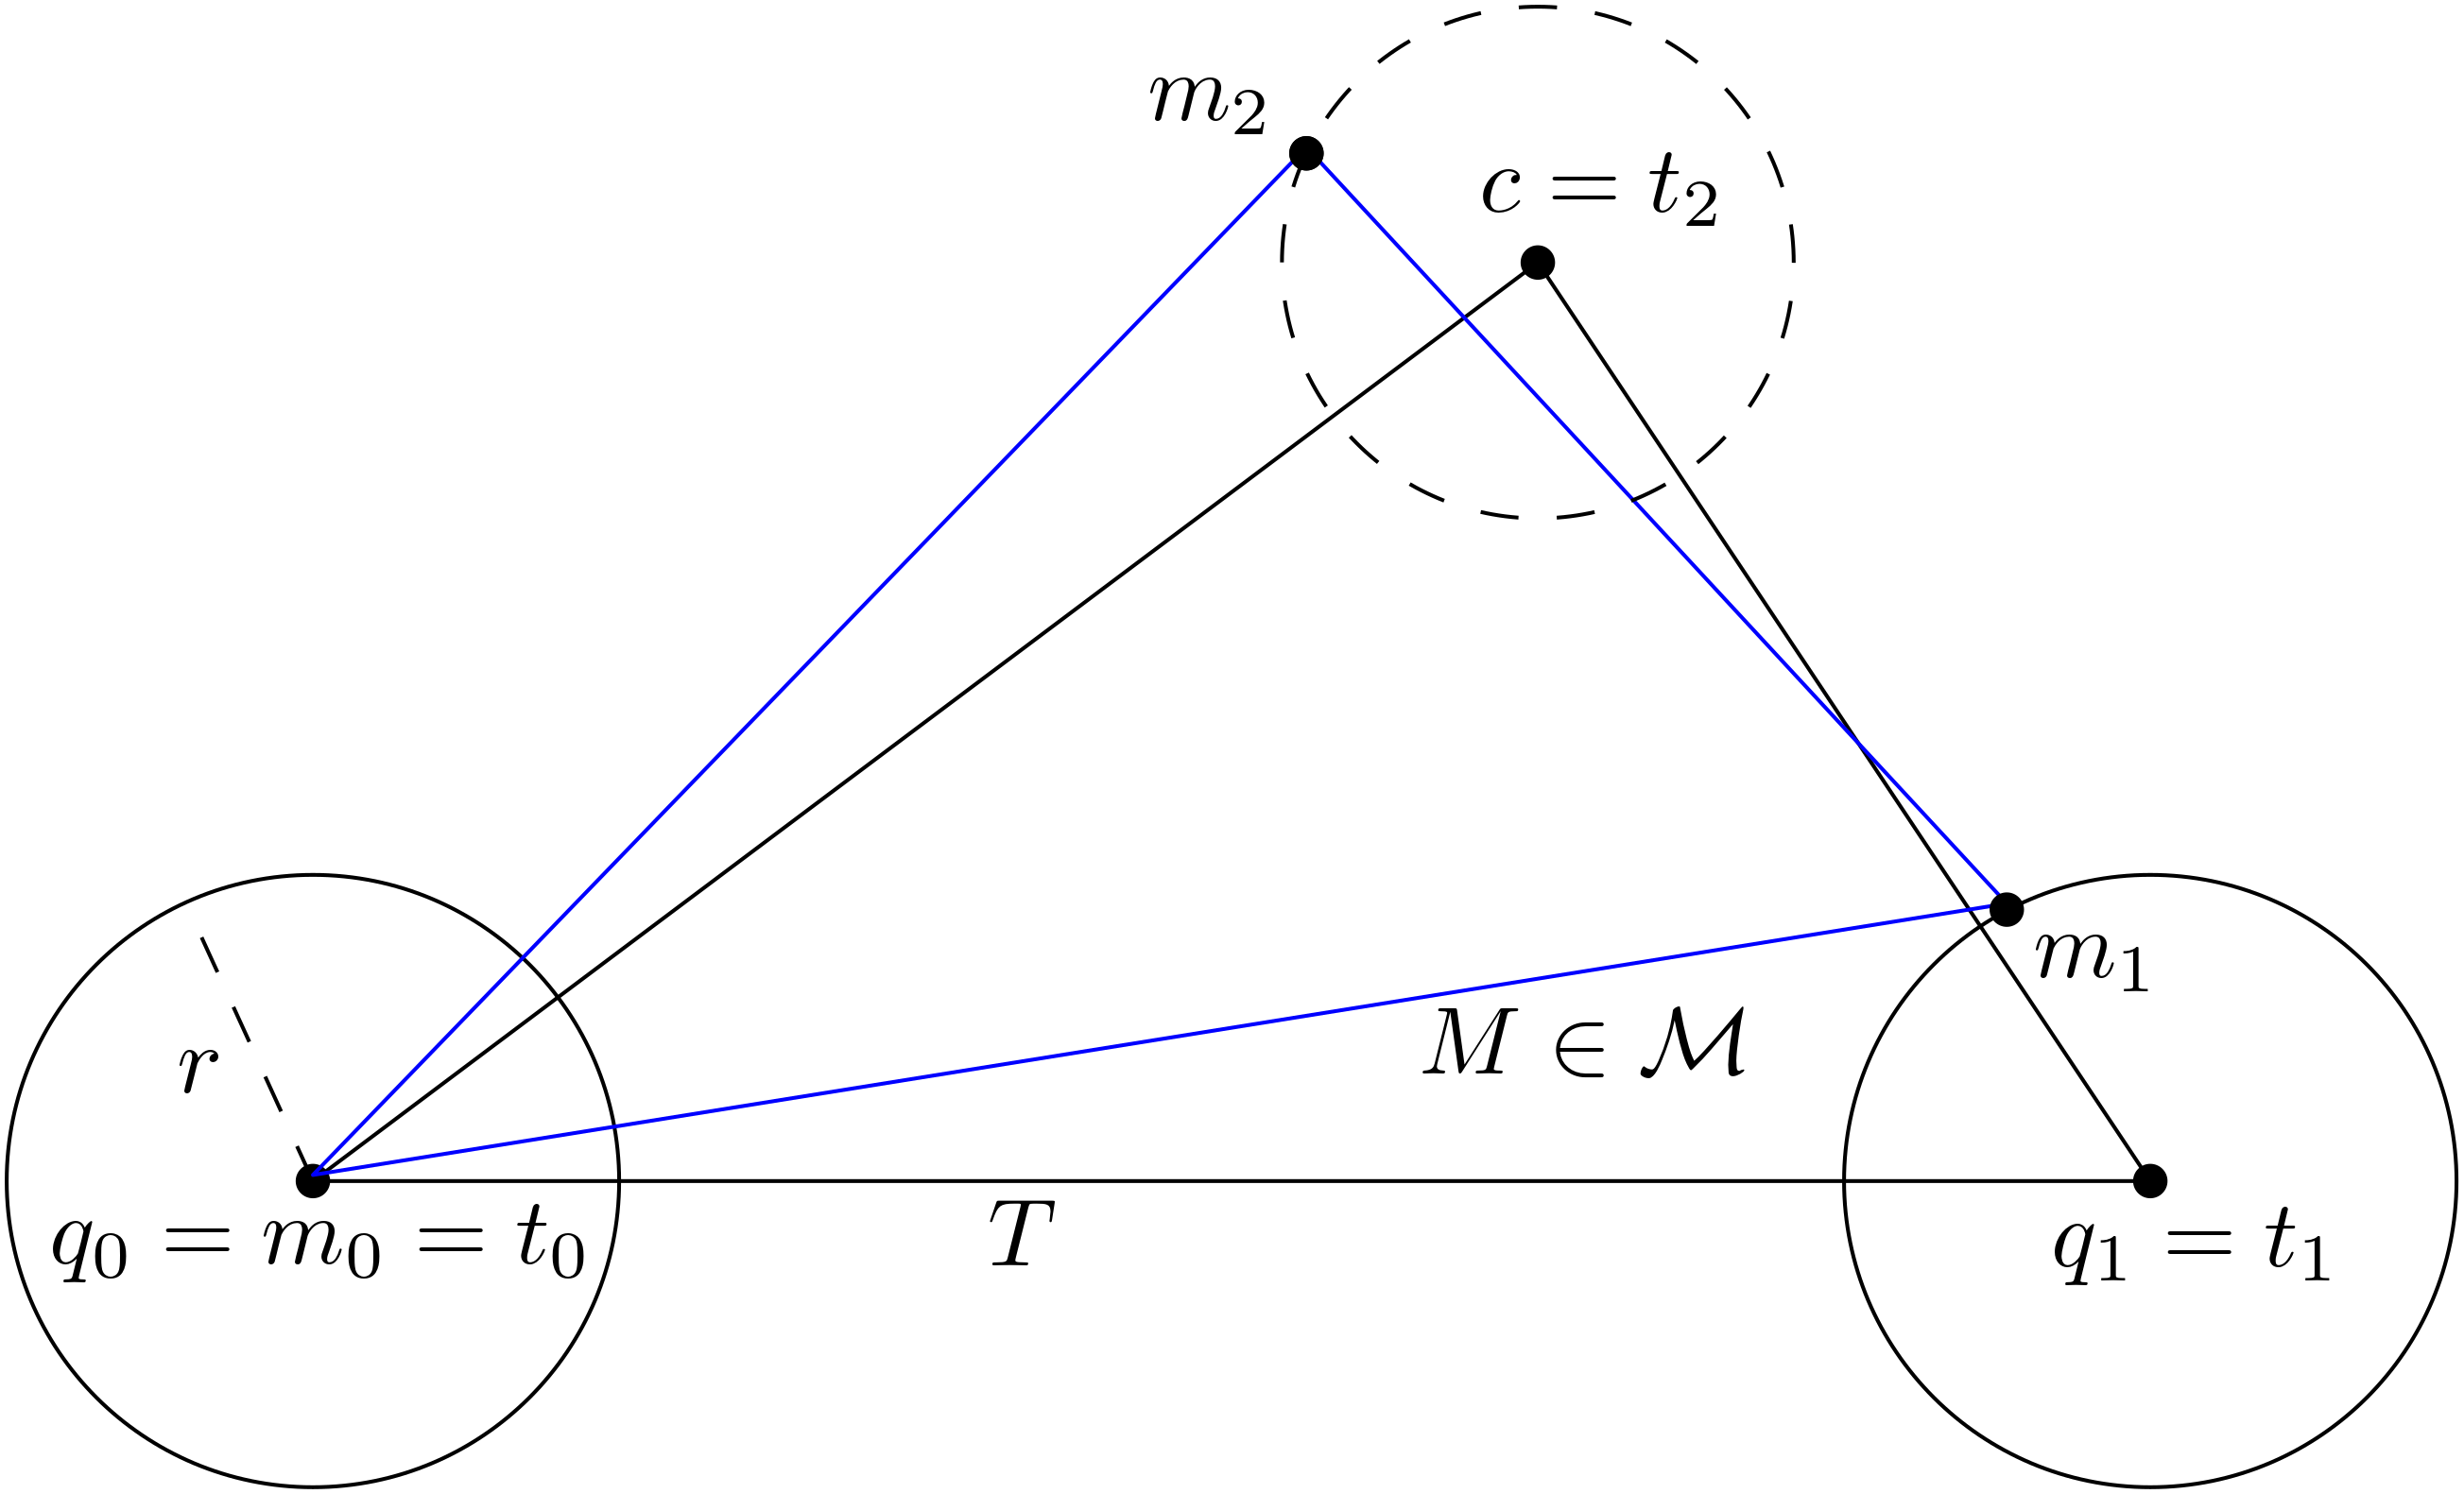
\includegraphics[width=\textwidth]{../media/replication_machine.png}
                \end{center}
            \end{column}
        \end{columns}
        
        \framebreak

        
        \begin{columns}
            \begin{column}{0.5\textwidth}
                \begin{proof}[\proofname\ (Cont.)]
                    Now consider the replication $M$ such that $m_1$
                    is colinear with $\overline{q_0q_1}$.

                    \bigskip
        
                    Observe that $k d(q_0, q_1) = d(q_0, q_1) + r$ and 
                    $k d(q_0, t_i) = d(q_1, t_1) + d(t_i, m_i)$. 

                    \bigskip
        
                    Solving the system of equations results in 
                    $d(t_i, m_i) = r \frac{d(q_0, t_i)}{d(q_0, q_1)}$.
                \end{proof}  
            \end{column}
            \begin{column}{0.5\textwidth}  %%<--- here
                \begin{center}
                    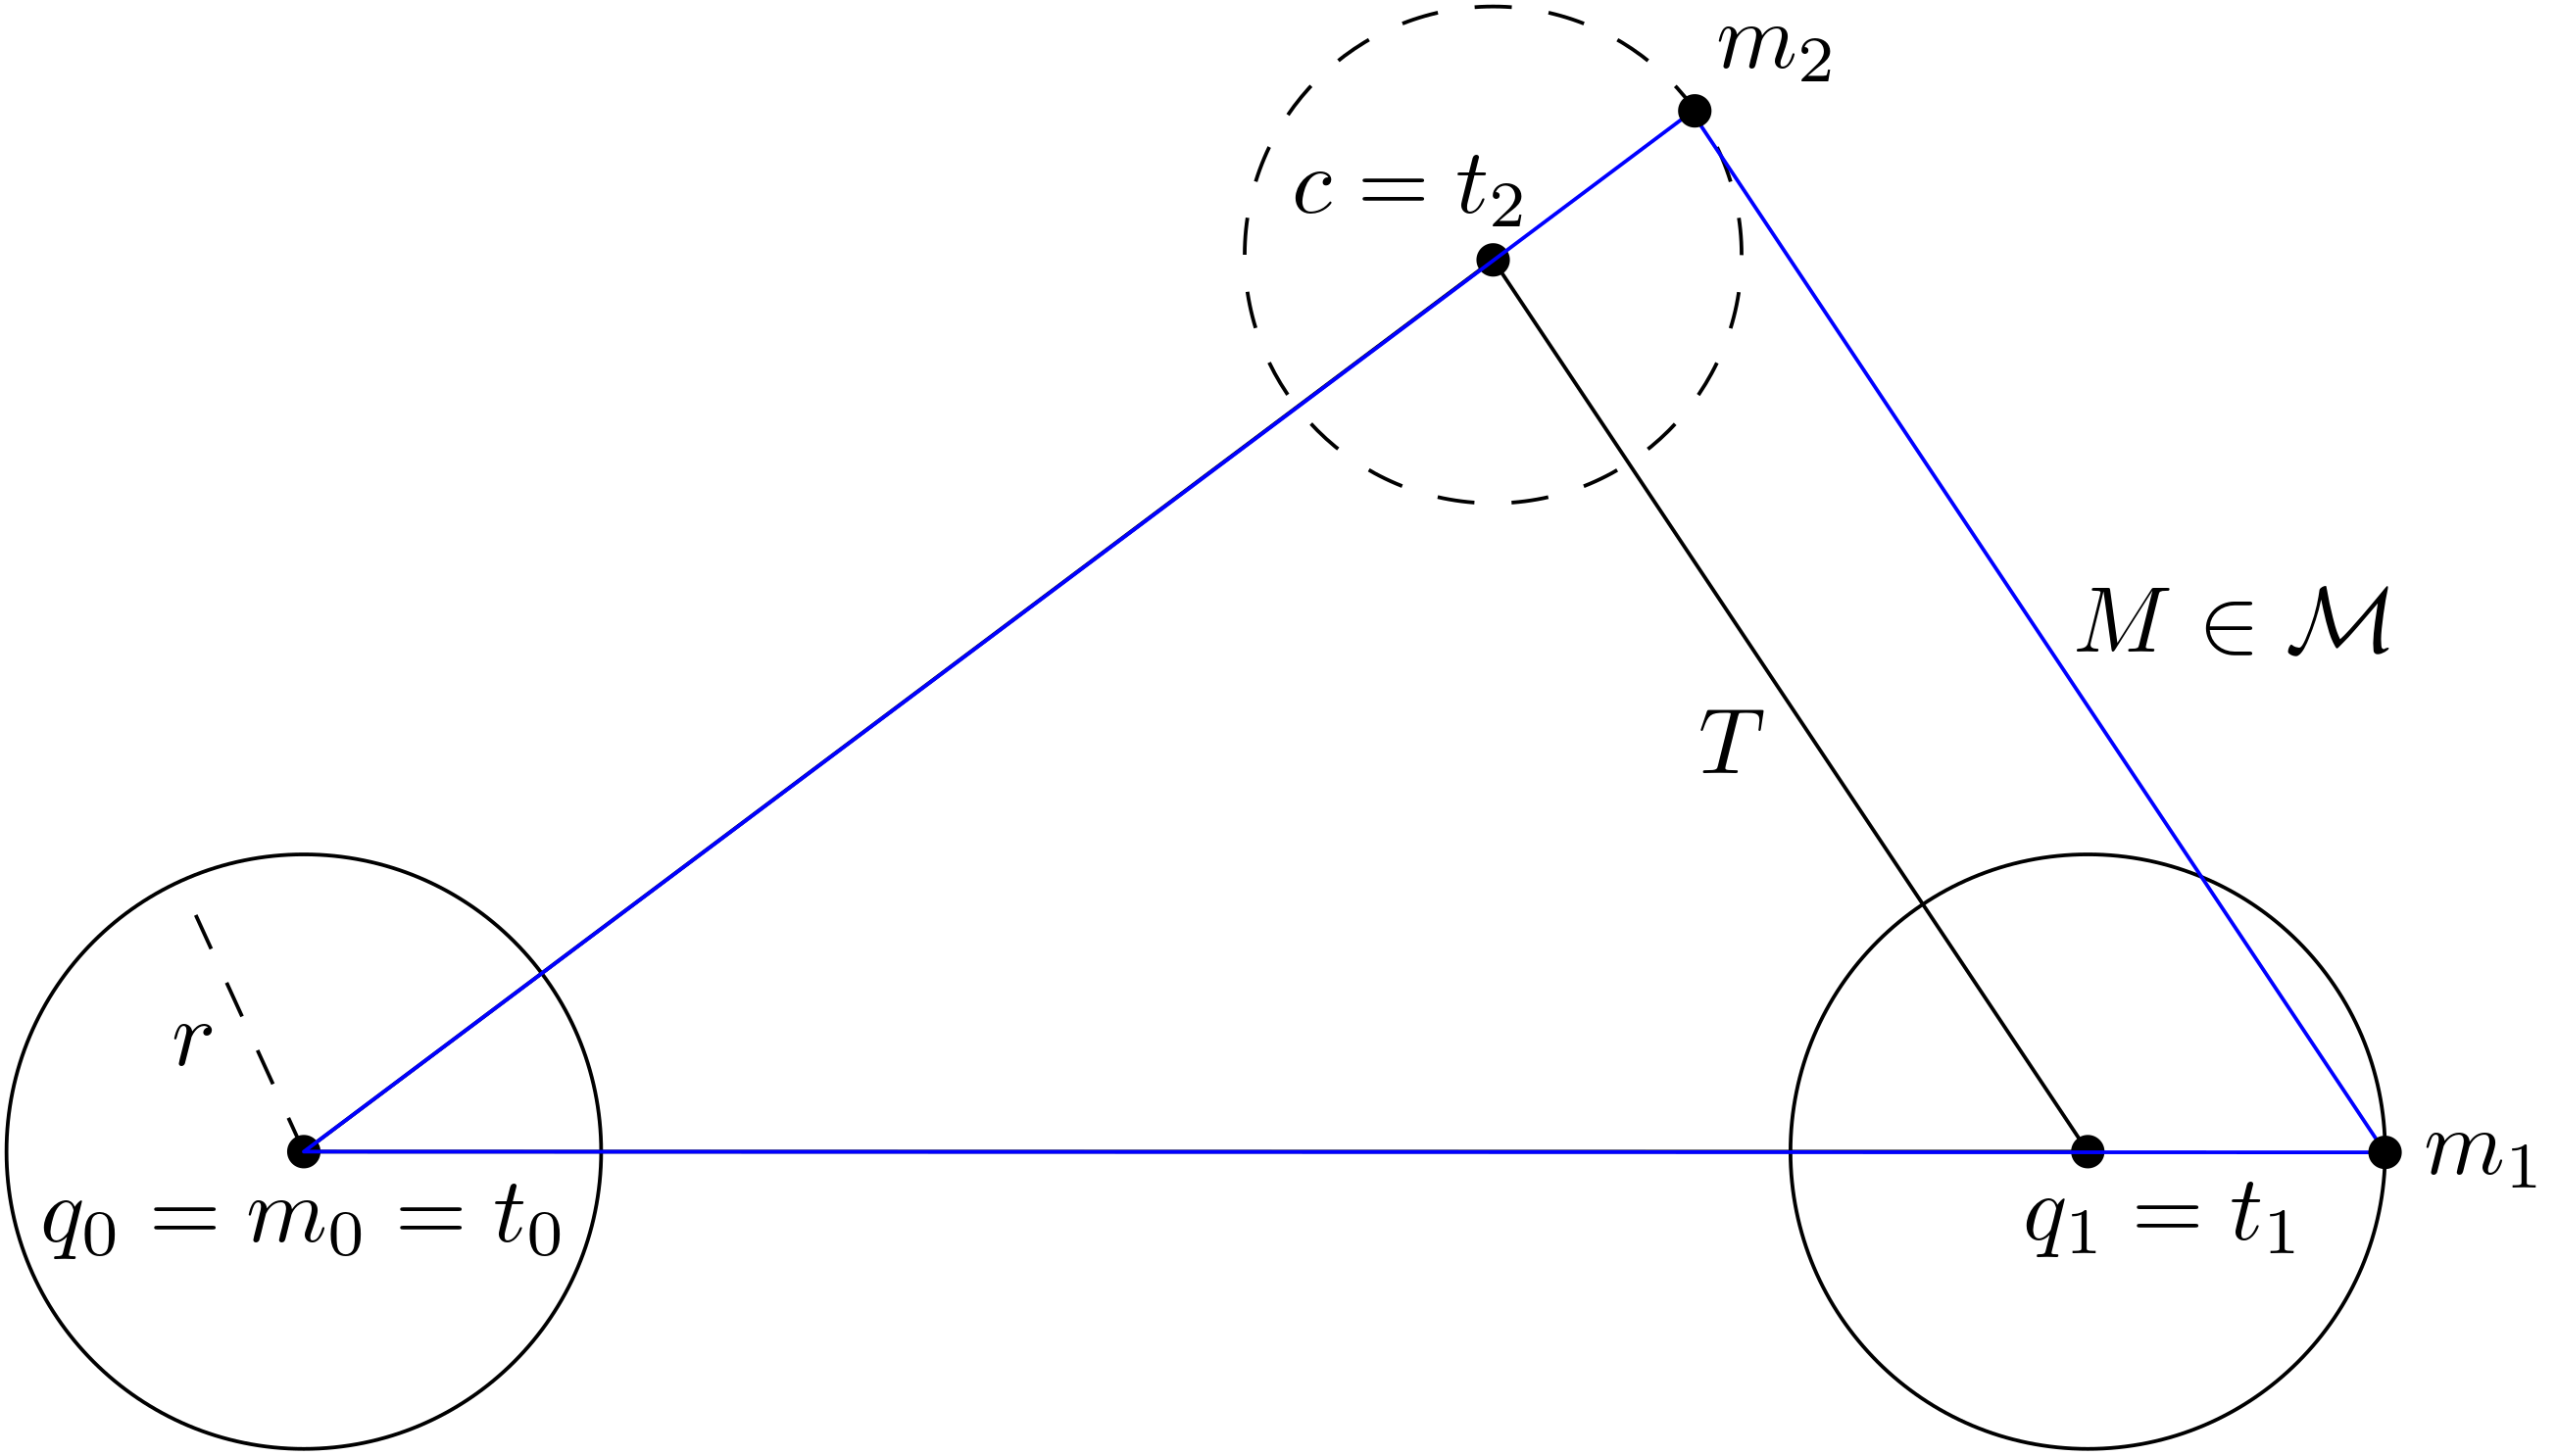
\includegraphics[width=\textwidth]{../media/replication_machine_radius.png}
                \end{center}
            \end{column}
        \end{columns}

    \end{frame}

    \begin{frame}[allowframebreaks]{Replication Spanner Circles}  
        
        Given a formation $P$ of size $n$, points $q_0$ and $q_1$, and a distance $r$.

        \begin{lemma}
            The $n$ sets of $i^{th}$ points in the replicated shapes are contained entirely in a closed disk centered at $t_i$ with radius 
            $r \frac{d(q_0, t_i) + d(q_1, t_i)}{d(q_0, q_1)}$.
        \end{lemma}

        \framebreak

        \begin{columns}
            \begin{column}{0.5\textwidth}
                \begin{proof}
                
                    Let $T = R_{Trivial}(P, q_0, q_1)$, 
                    $\mathcal{M} = R_{Machine}(\{p_1, p_0, p_2, \ldots, p_{n-1}\}, q, p, r)$, and 
                    $\mathcal{S} = R_{Span}(P, p, q, r)$

                    \bigskip

                    Observe the center of the $i^{th}$ circle spanned by $S$
                    is in the $i^{th}$ circle spanned by $\mathcal{M}$. 
                    Therefore, $t_i$ is a center-of-centers. 
                    
                    The radius can then be computed:
                 
                    \begin{center}
                       $d(t_i, m_i) + d(m_i, s_i) = r \frac{d(q_0, t_i) + d(q_1, t_i)}{d(q_0, q_1)}$
                    \end{center}
                 \end{proof} 
            \end{column}
            \begin{column}{0.5\textwidth}  %%<--- here
                \begin{center}
                    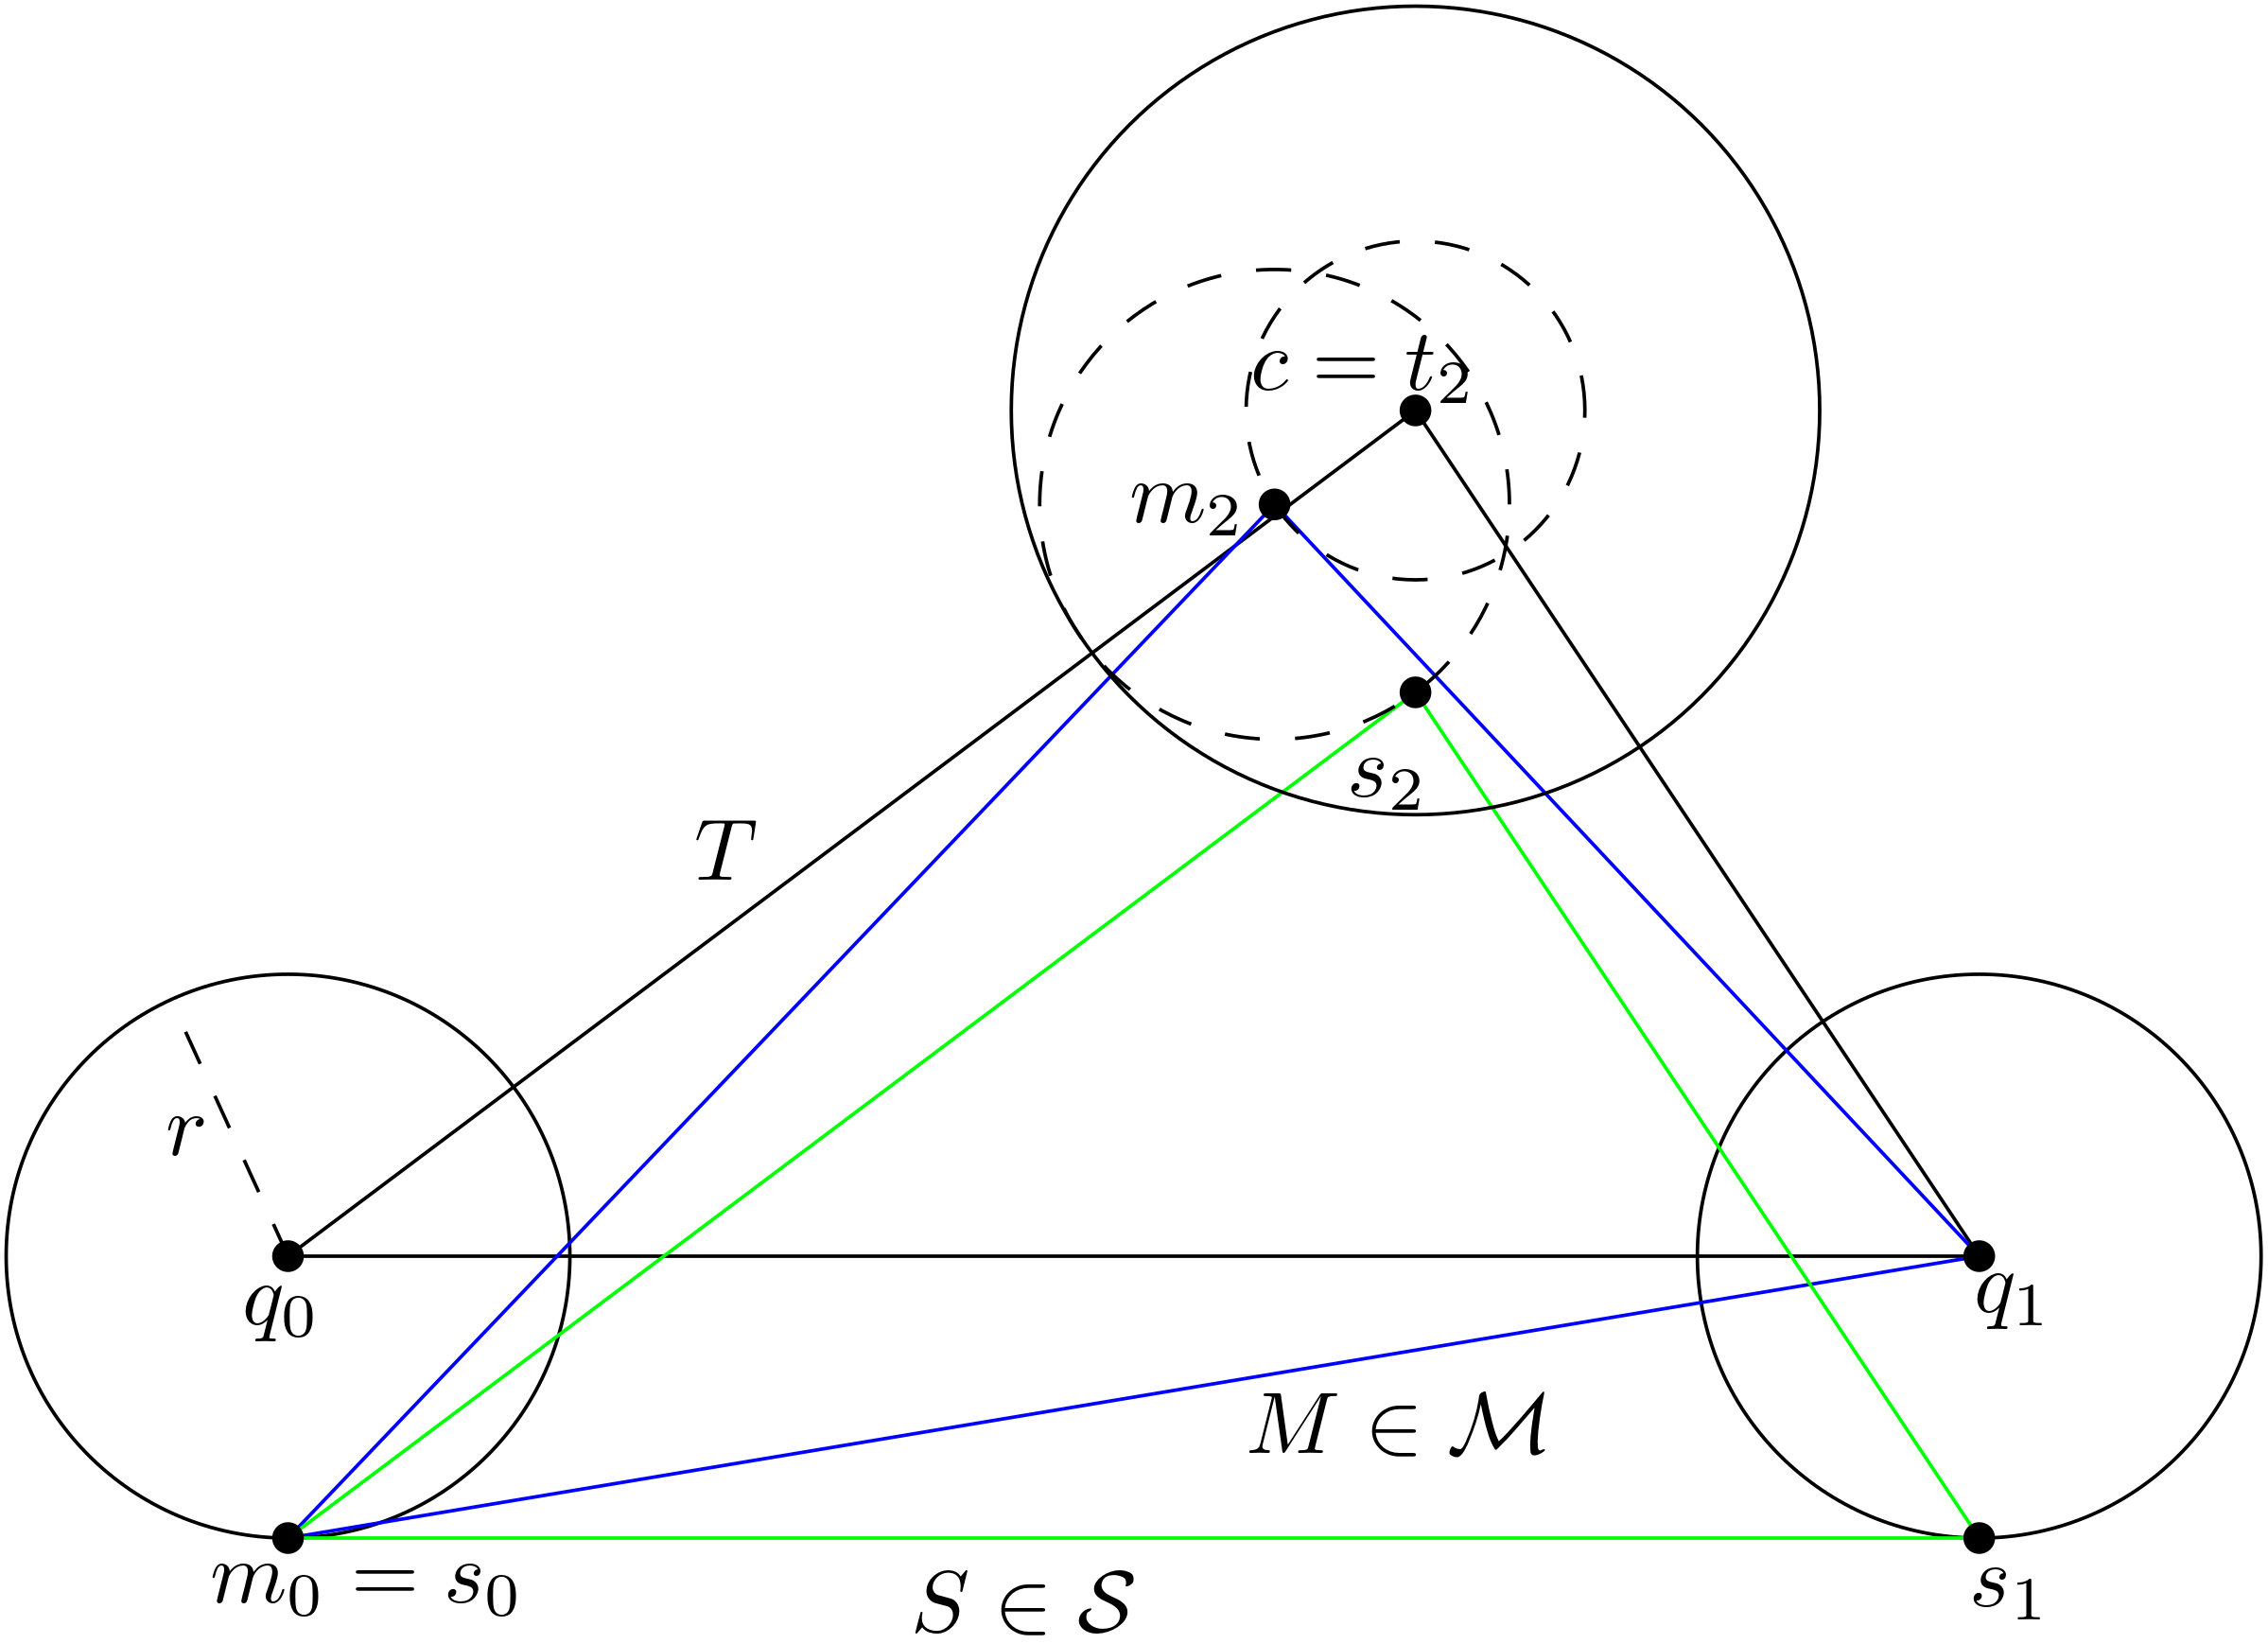
\includegraphics[width=\textwidth]{../media/replication_spanner.png}
                \end{center}
            \end{column}
        \end{columns}
    
    \end{frame}

    \section{Forming Triangles}

    \begin{frame}{Construction}
        \framesubtitle{Step 1: Trivial Replications}
        \begin{columns}
            \begin{column}{0.5\textwidth}
                Given the initial positions $P$ and pattern $S$, consider all of the trivial replications of $S$ on $P$, 
                $t^i = T(\{s_{i+1}, s_{i+2}, s_i\}, p_{i+1}, p_{i+2})_i$ 
                for $0 \leq i \leq 2$.
            \end{column}
            \begin{column}{0.5\textwidth}  %%<--- here
                \begin{center}
                    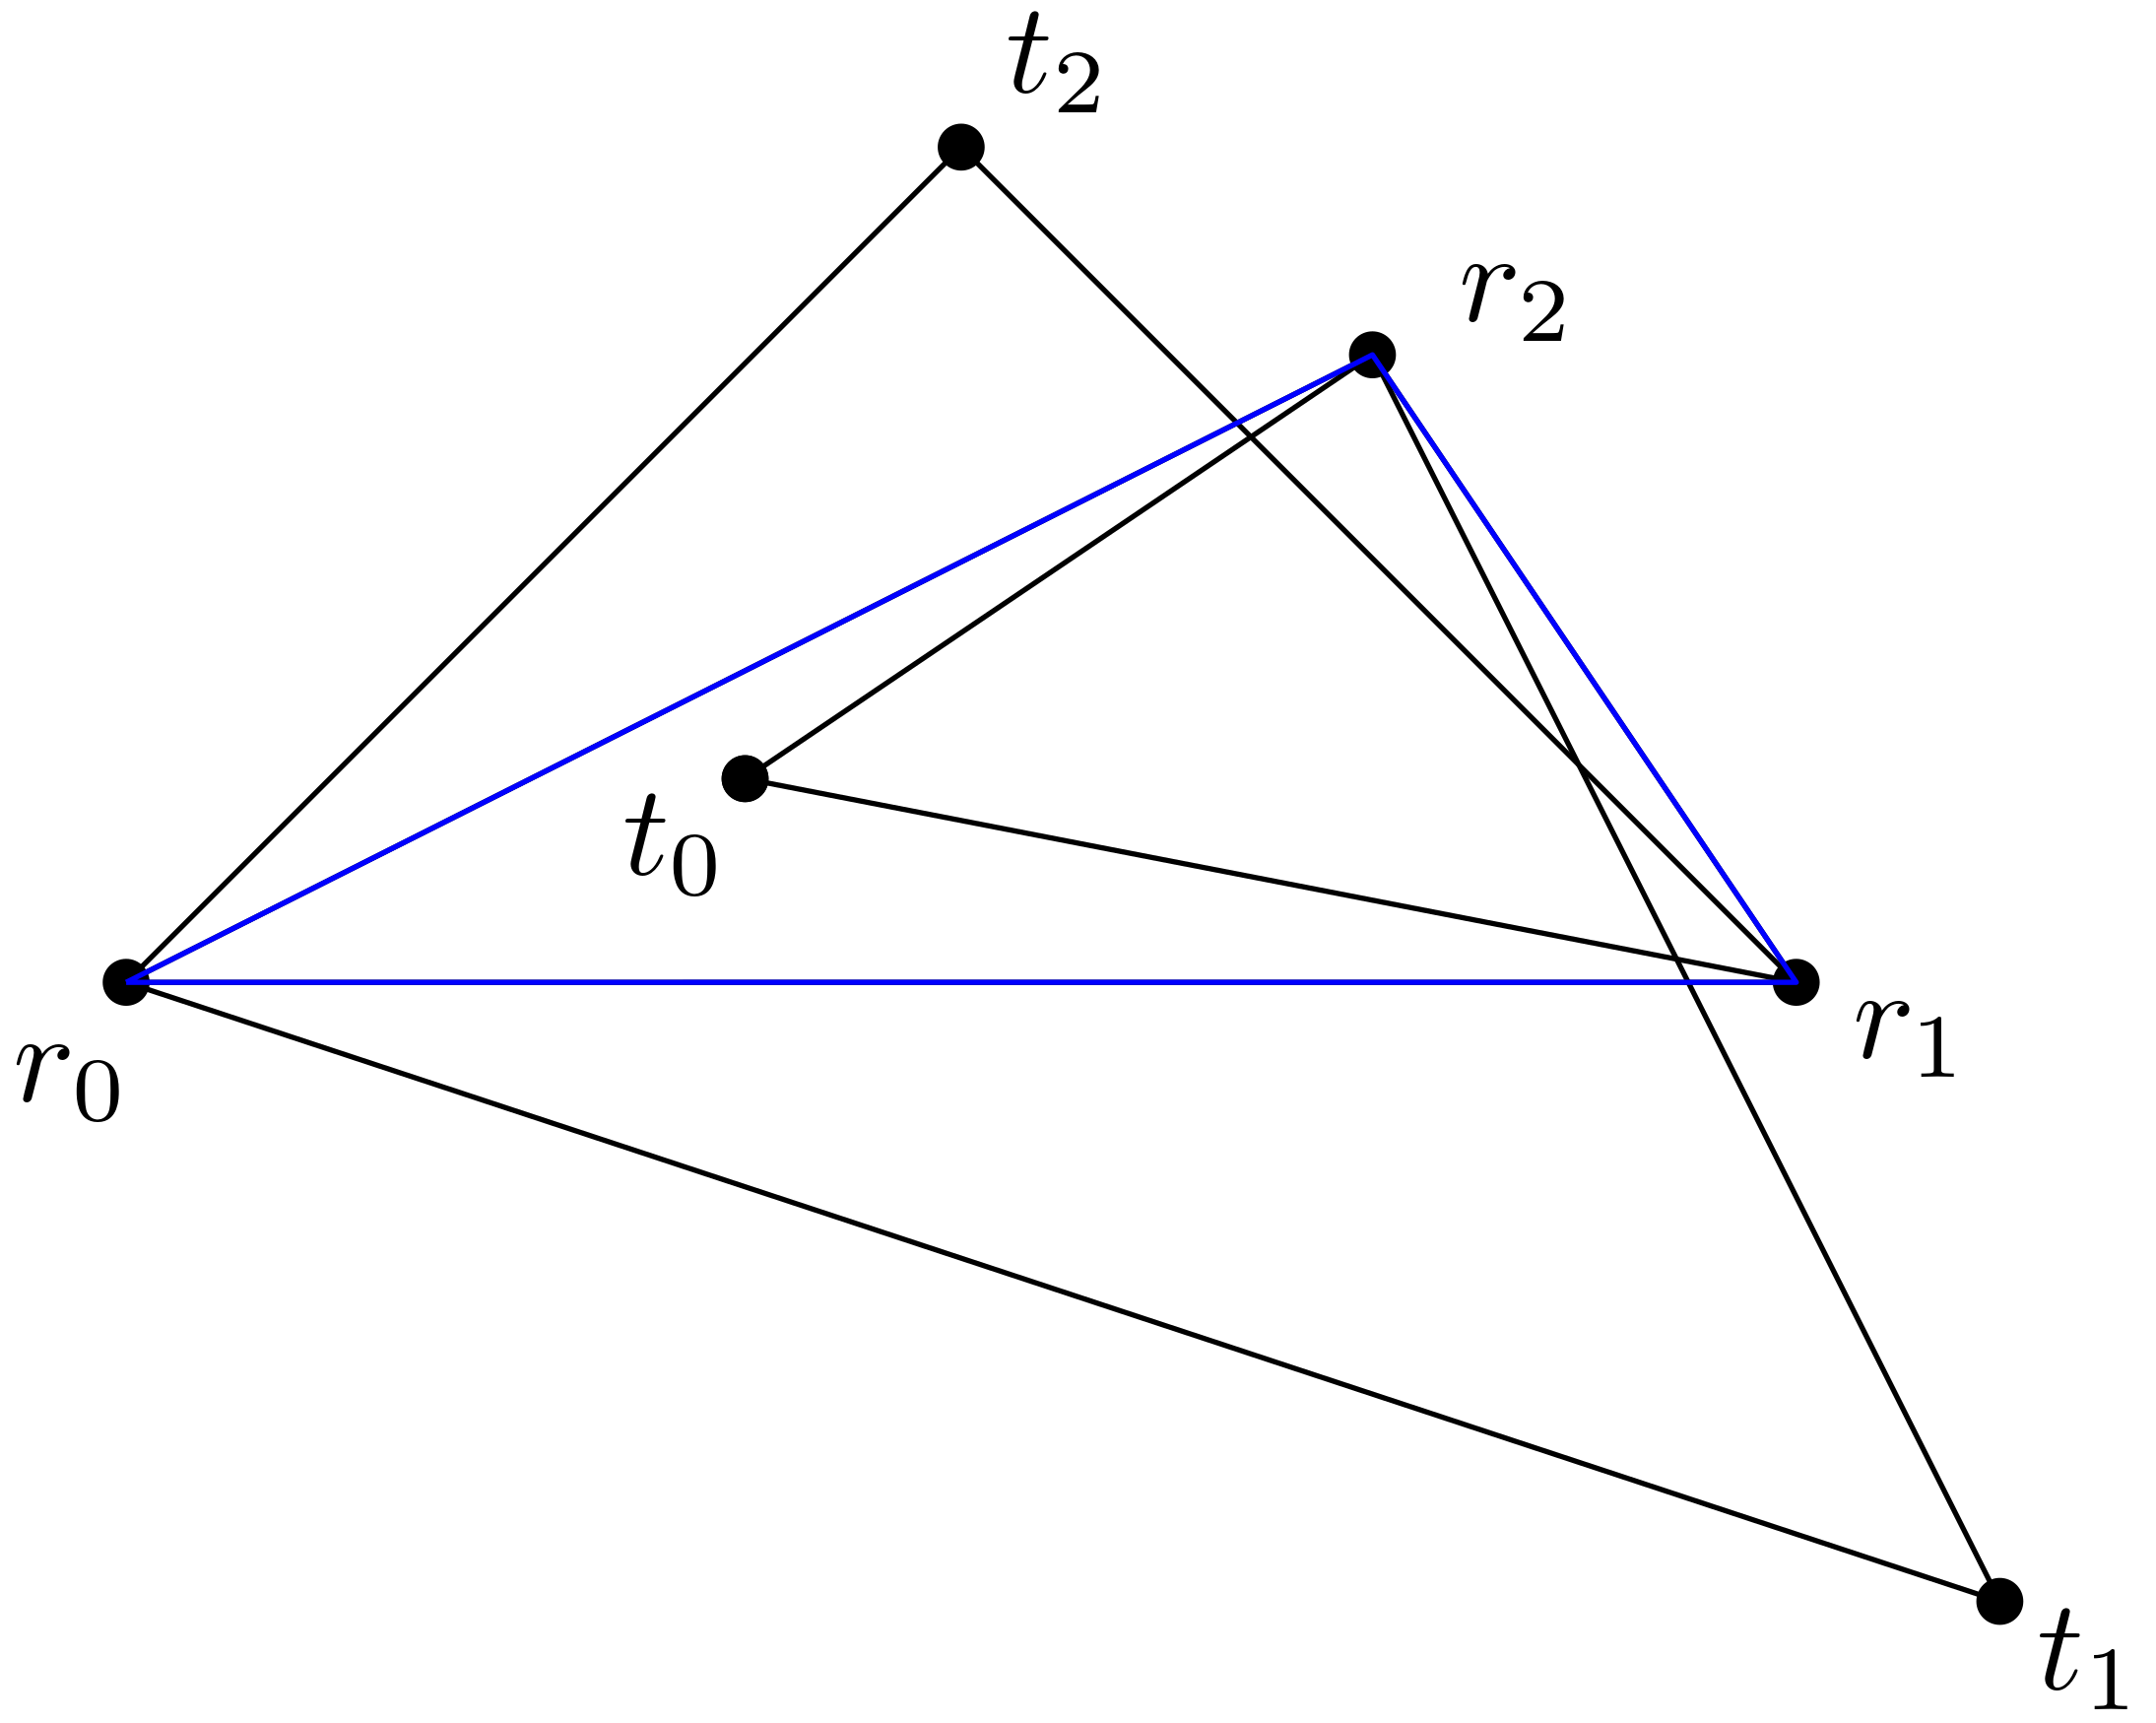
\includegraphics[width=\textwidth]{../media/construction_1.png}
                \end{center}
            \end{column}
        \end{columns}
    \end{frame}

    \begin{frame}{Construction}
        \framesubtitle{Step 2: Replication Spanners}
        \begin{columns}
            \begin{column}{0.5\textwidth}
                Then, for some unknown $r$, consider the replication spanners
                $R_{SPAN}(\{s_{i}, s_{i+1}, s_{i+2}\}, p_i, p_{i+1}, r)$
                for $0 \leq i \leq 2$.

                \bigskip

                Notice that for some $r$ there exists a single point of intersection, $q_i$, between $C(p_i, r)$ and the $i^{th}$ circle generated by $\mathcal{S}$. 
                
            \end{column}
            \begin{column}{0.5\textwidth}  %%<--- here
                \begin{center}
                    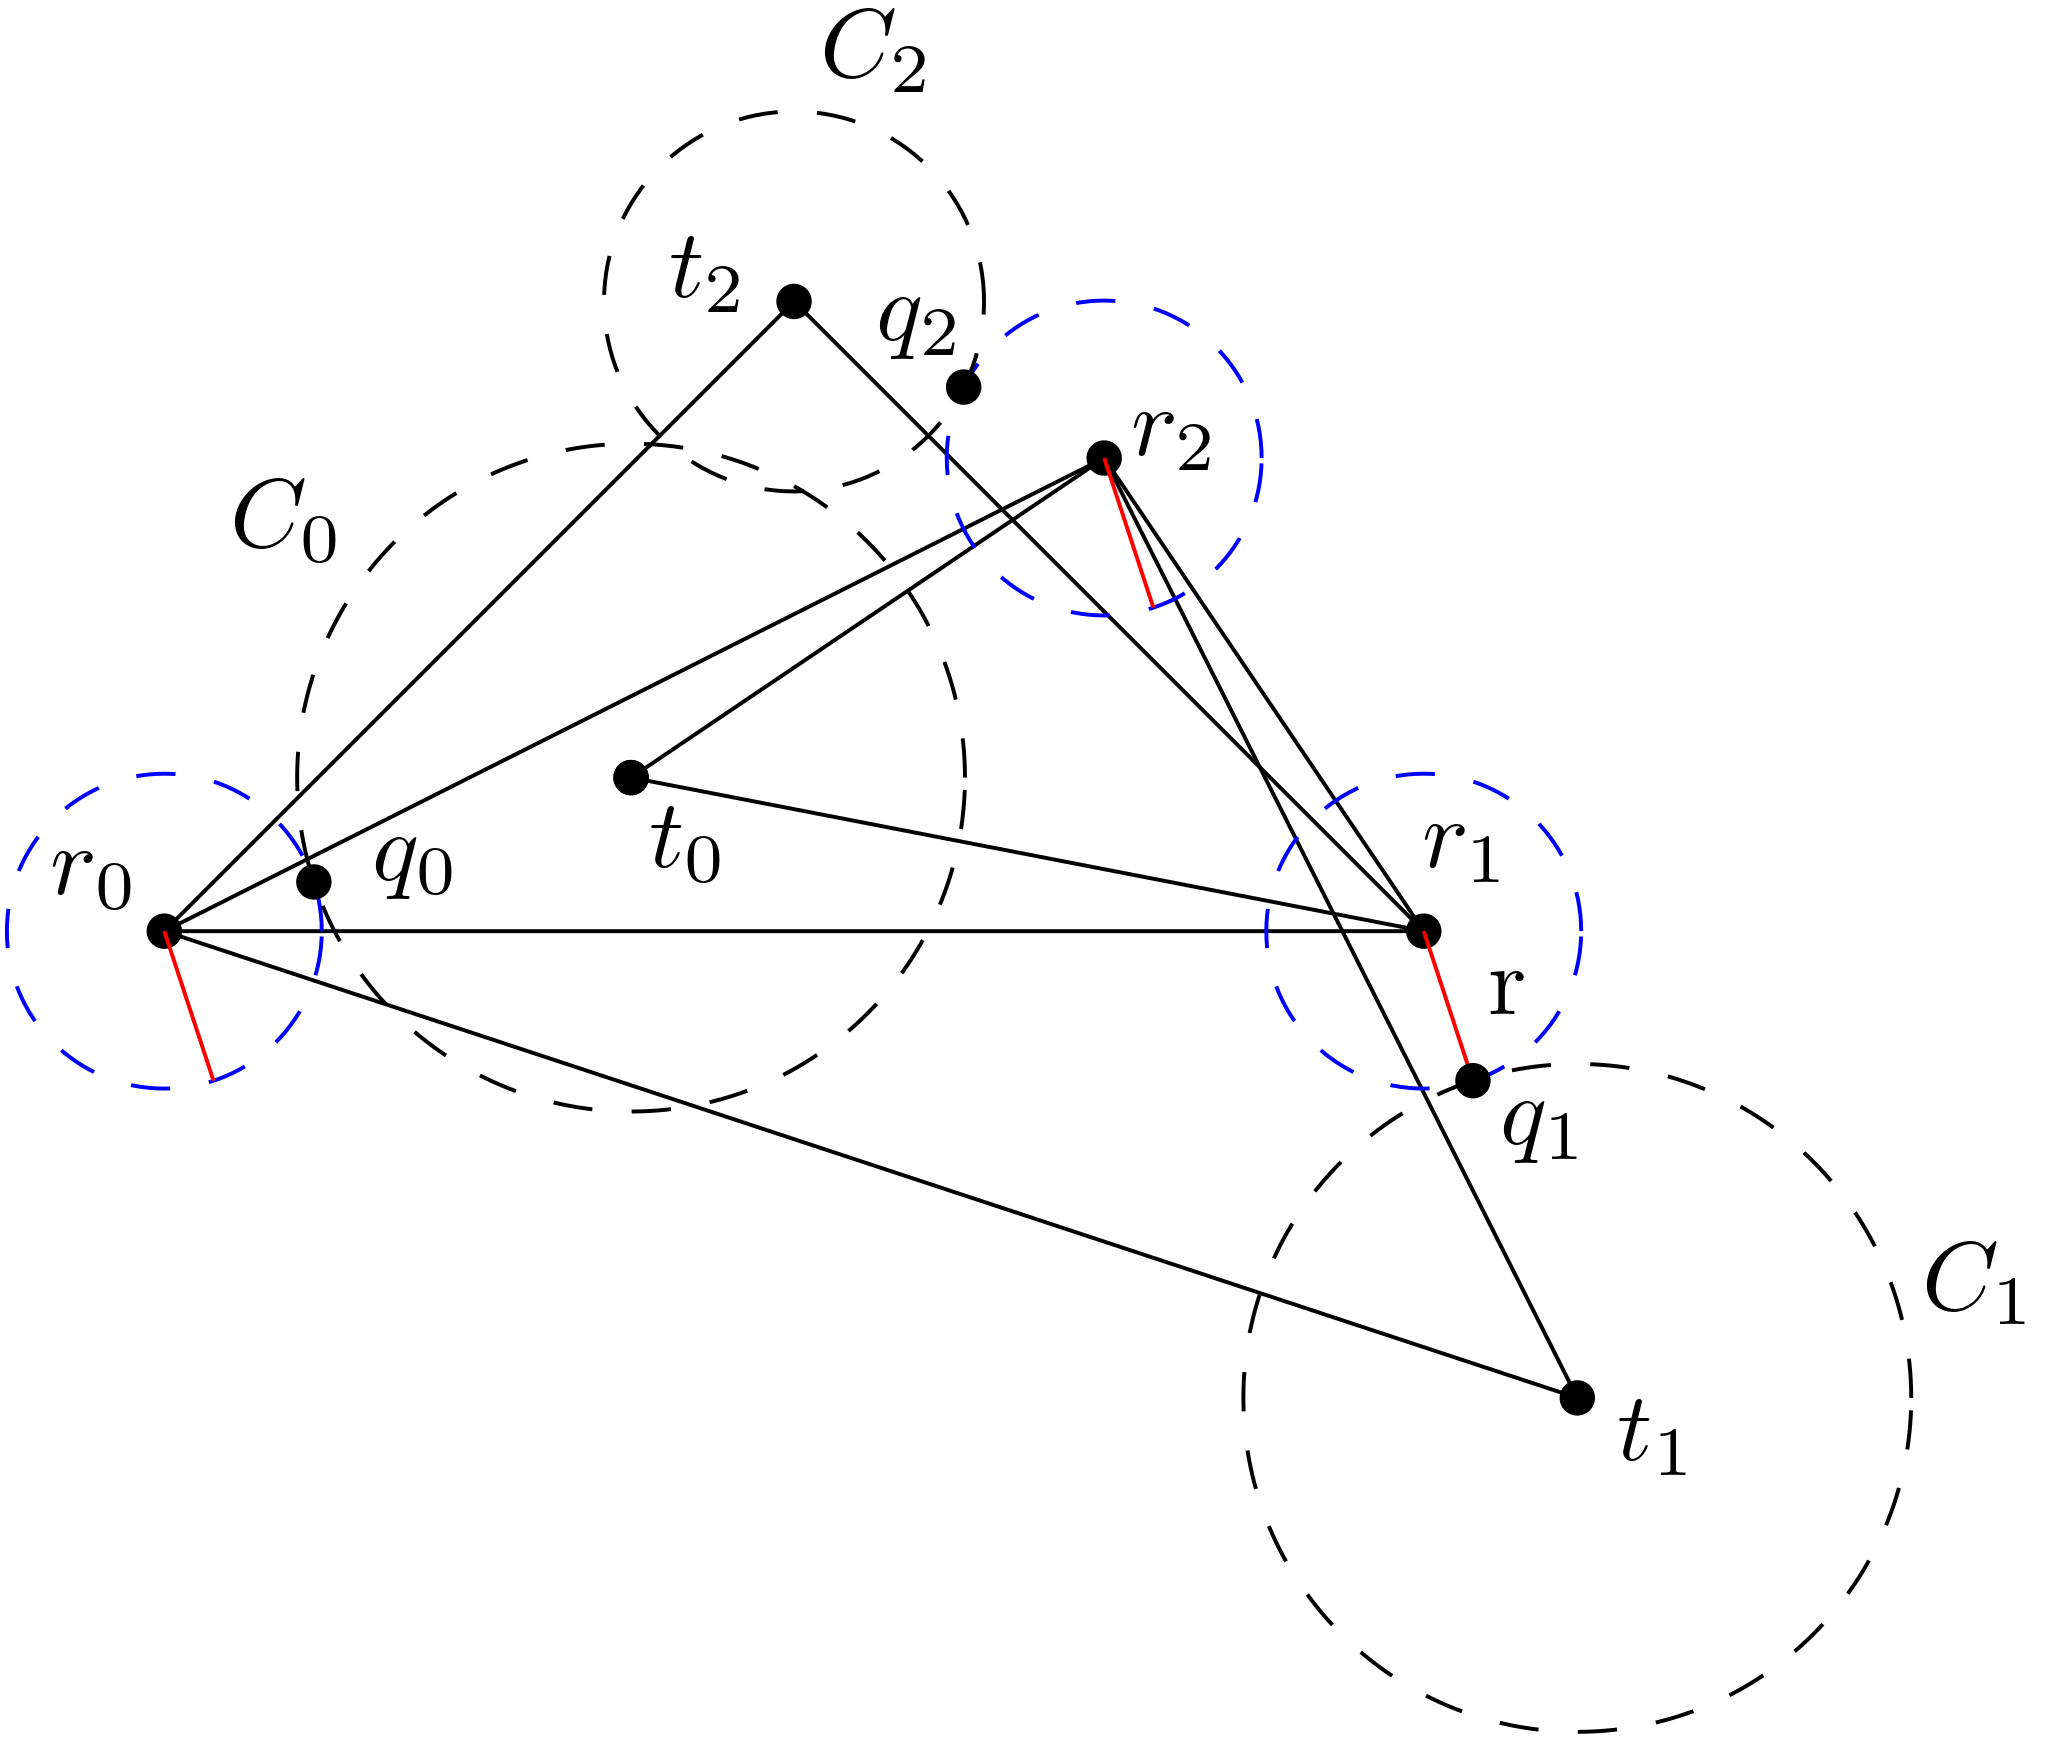
\includegraphics[width=\textwidth]{../media/construction_2.png}
                \end{center}
            \end{column}
        \end{columns}
    \end{frame}

    \begin{frame}{Construction}
        \framesubtitle{Step 3: Compute the Radius}
        Then $r$ can be computed algebraically:

        \begin{align*}
            d(p_i, t_i) - r &= r \frac{d(s_i, s_{i+1}) + d(s_i, s_{i+2})}{d(s_{i+1}, s_{i+2})} \\ 
            d(p_i, t_i) &= r \left( \frac{d(s_i, s_{i+1}) + d(s_i, s_{i+2})}{d(s_{i+1}, s_{i+2})} + 1 \right) \\ 
            d(p_i, t_i) &= r \left( \frac{d(s_i, s_{i+1}) + d(s_i, s_{i+2}) + d(s_{i+1}, s_{i+2})}{d(s_{i+1}, s_{i+2})} \right) \\
            d(p_i, t_i) &= \frac{r}{d(s_{i+1}, s_{i+2})} \\
            r &= d(p_i, t_i) ~ d(s_{i+1}, s_{i+2})
        \end{align*}
    \end{frame} 

    \begin{frame}[allowframebreaks]{Solution Validity}
        \begin{lemma}
            The target formation $Q = \{q_0, q_1, q_2\}$ is similar to the desired pattern $S$.
        \end{lemma}

        \framebreak

        \begin{columns}
            \begin{column}{0.5\textwidth}
                \begin{proof}
                   Note that given $q_2$, there must exist a unique pair of points 
                   $q^\prime_0 \in C(p_0, r)$ and 
                   $q^\prime_1 \in C(p_1, r)$ such that 
                   $Q^\prime=\{q^\prime_0, q^\prime_1, q_2\} \sim S$. 

                   \bigskip
                   
                   Suppose $q^\prime_1 \neq q_1$. This implies 
                   $q^\prime_1 \not\in D \left( p^\prime_1, r \frac{d(q_0, p^\prime_1) + d(q_1, p^\prime_1)} {d(q_0, q_1)} \right)$.

                   \bigskip

                   This is a contradiction.
                \end{proof}
                
            \end{column}
            \begin{column}{0.5\textwidth}  %%<--- here
                \begin{center}
                    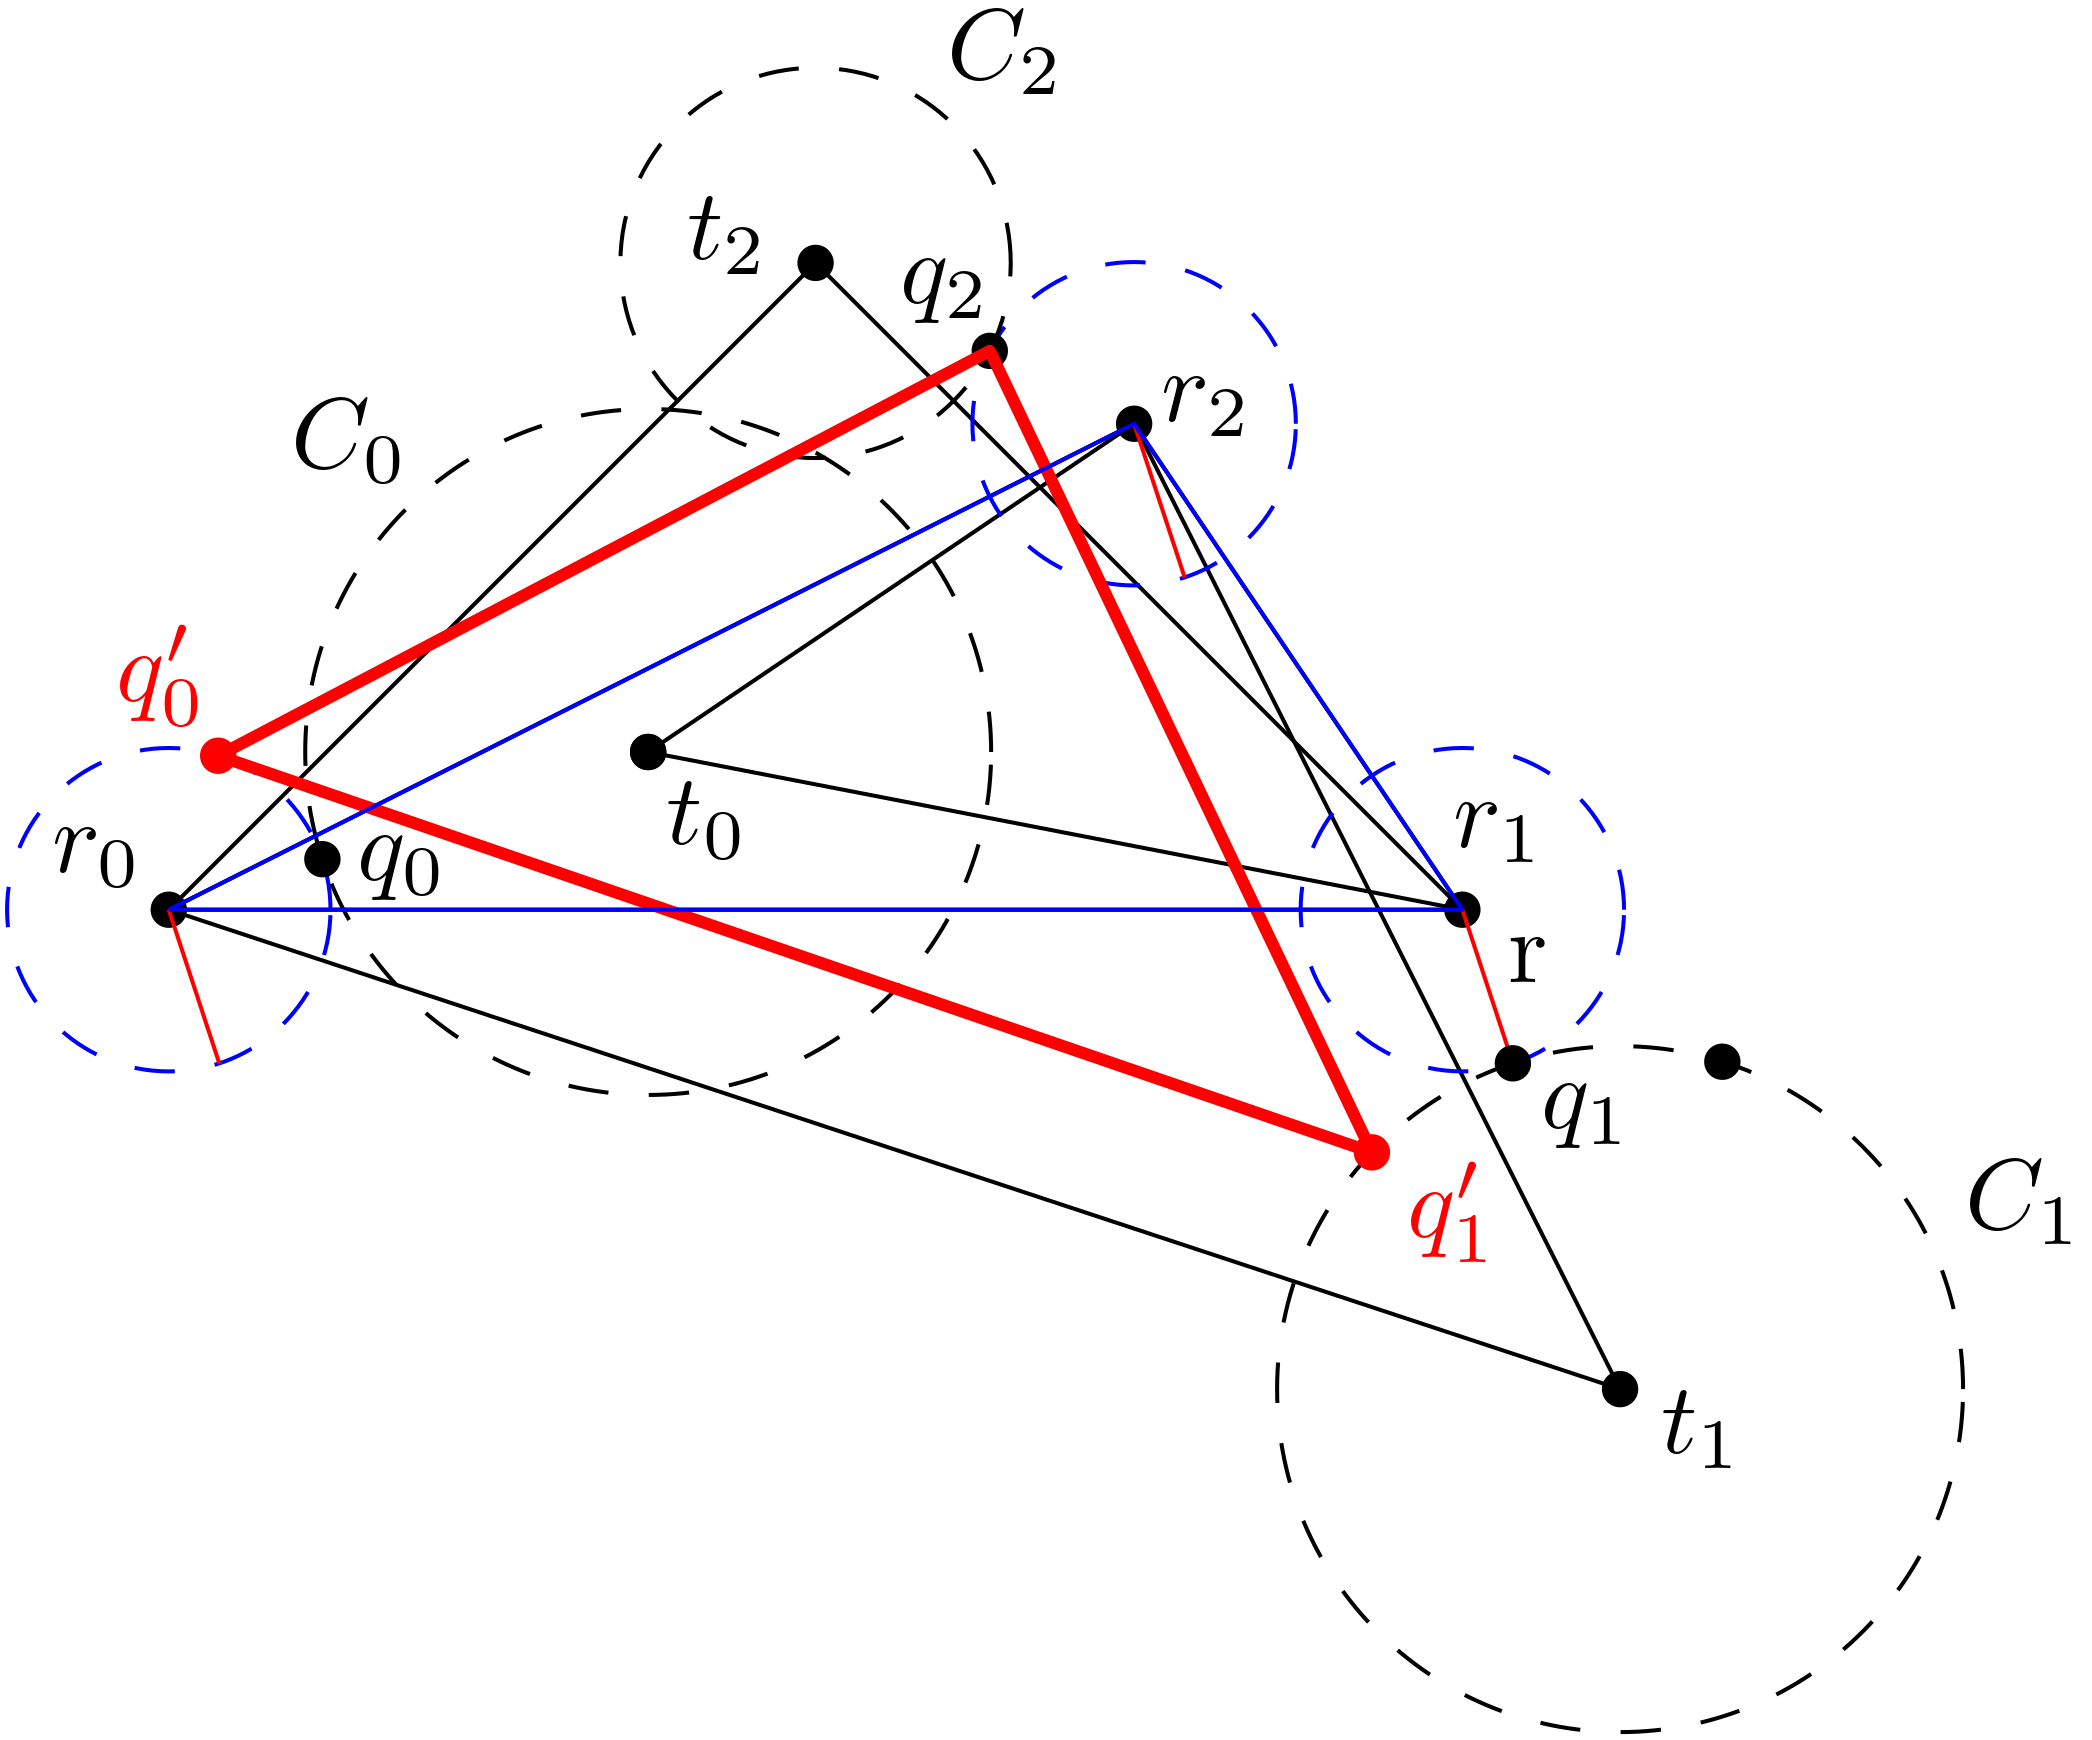
\includegraphics[width=\textwidth]{../media/construction_valid.png}
                \end{center}
            \end{column}
        \end{columns}
        

    \end{frame}

    \note{
        Fact follows from the results of the translation spanner defined above. \\
        A similar argument can be made to prove $q_0 = q^\prime_0$
    }

    \begin{frame}[allowframebreaks]{Solution Optimality}
        \begin{lemma}
            The target formation $Q = \{q_0, q_1, q_2\}$ is the optimal solution for the initial positions $P$.
        \end{lemma}

        \framebreak

        \begin{columns}
            \begin{column}{0.5\textwidth}
                \begin{proofs}
                    Let $r^\prime$ be some distance arbitrarily smaller than $r$.
                    Let $\mathcal{S}=R_{Span}(\{s_{i+1}, s_{i+2}, s_i\}, p_{i+1}, p_{i+2}, r^\prime)$.
                    
                    \bigskip

                    \textbf{Recall}: $\mathcal{S}$ is the set of all formations similar to $P$ such that $r_{i+1}$ and $r_{i+2}$ travel distance $r$.
                \end{proofs}
                
            \end{column}
            \begin{column}{0.5\textwidth}  %%<--- here
                \begin{center}
                    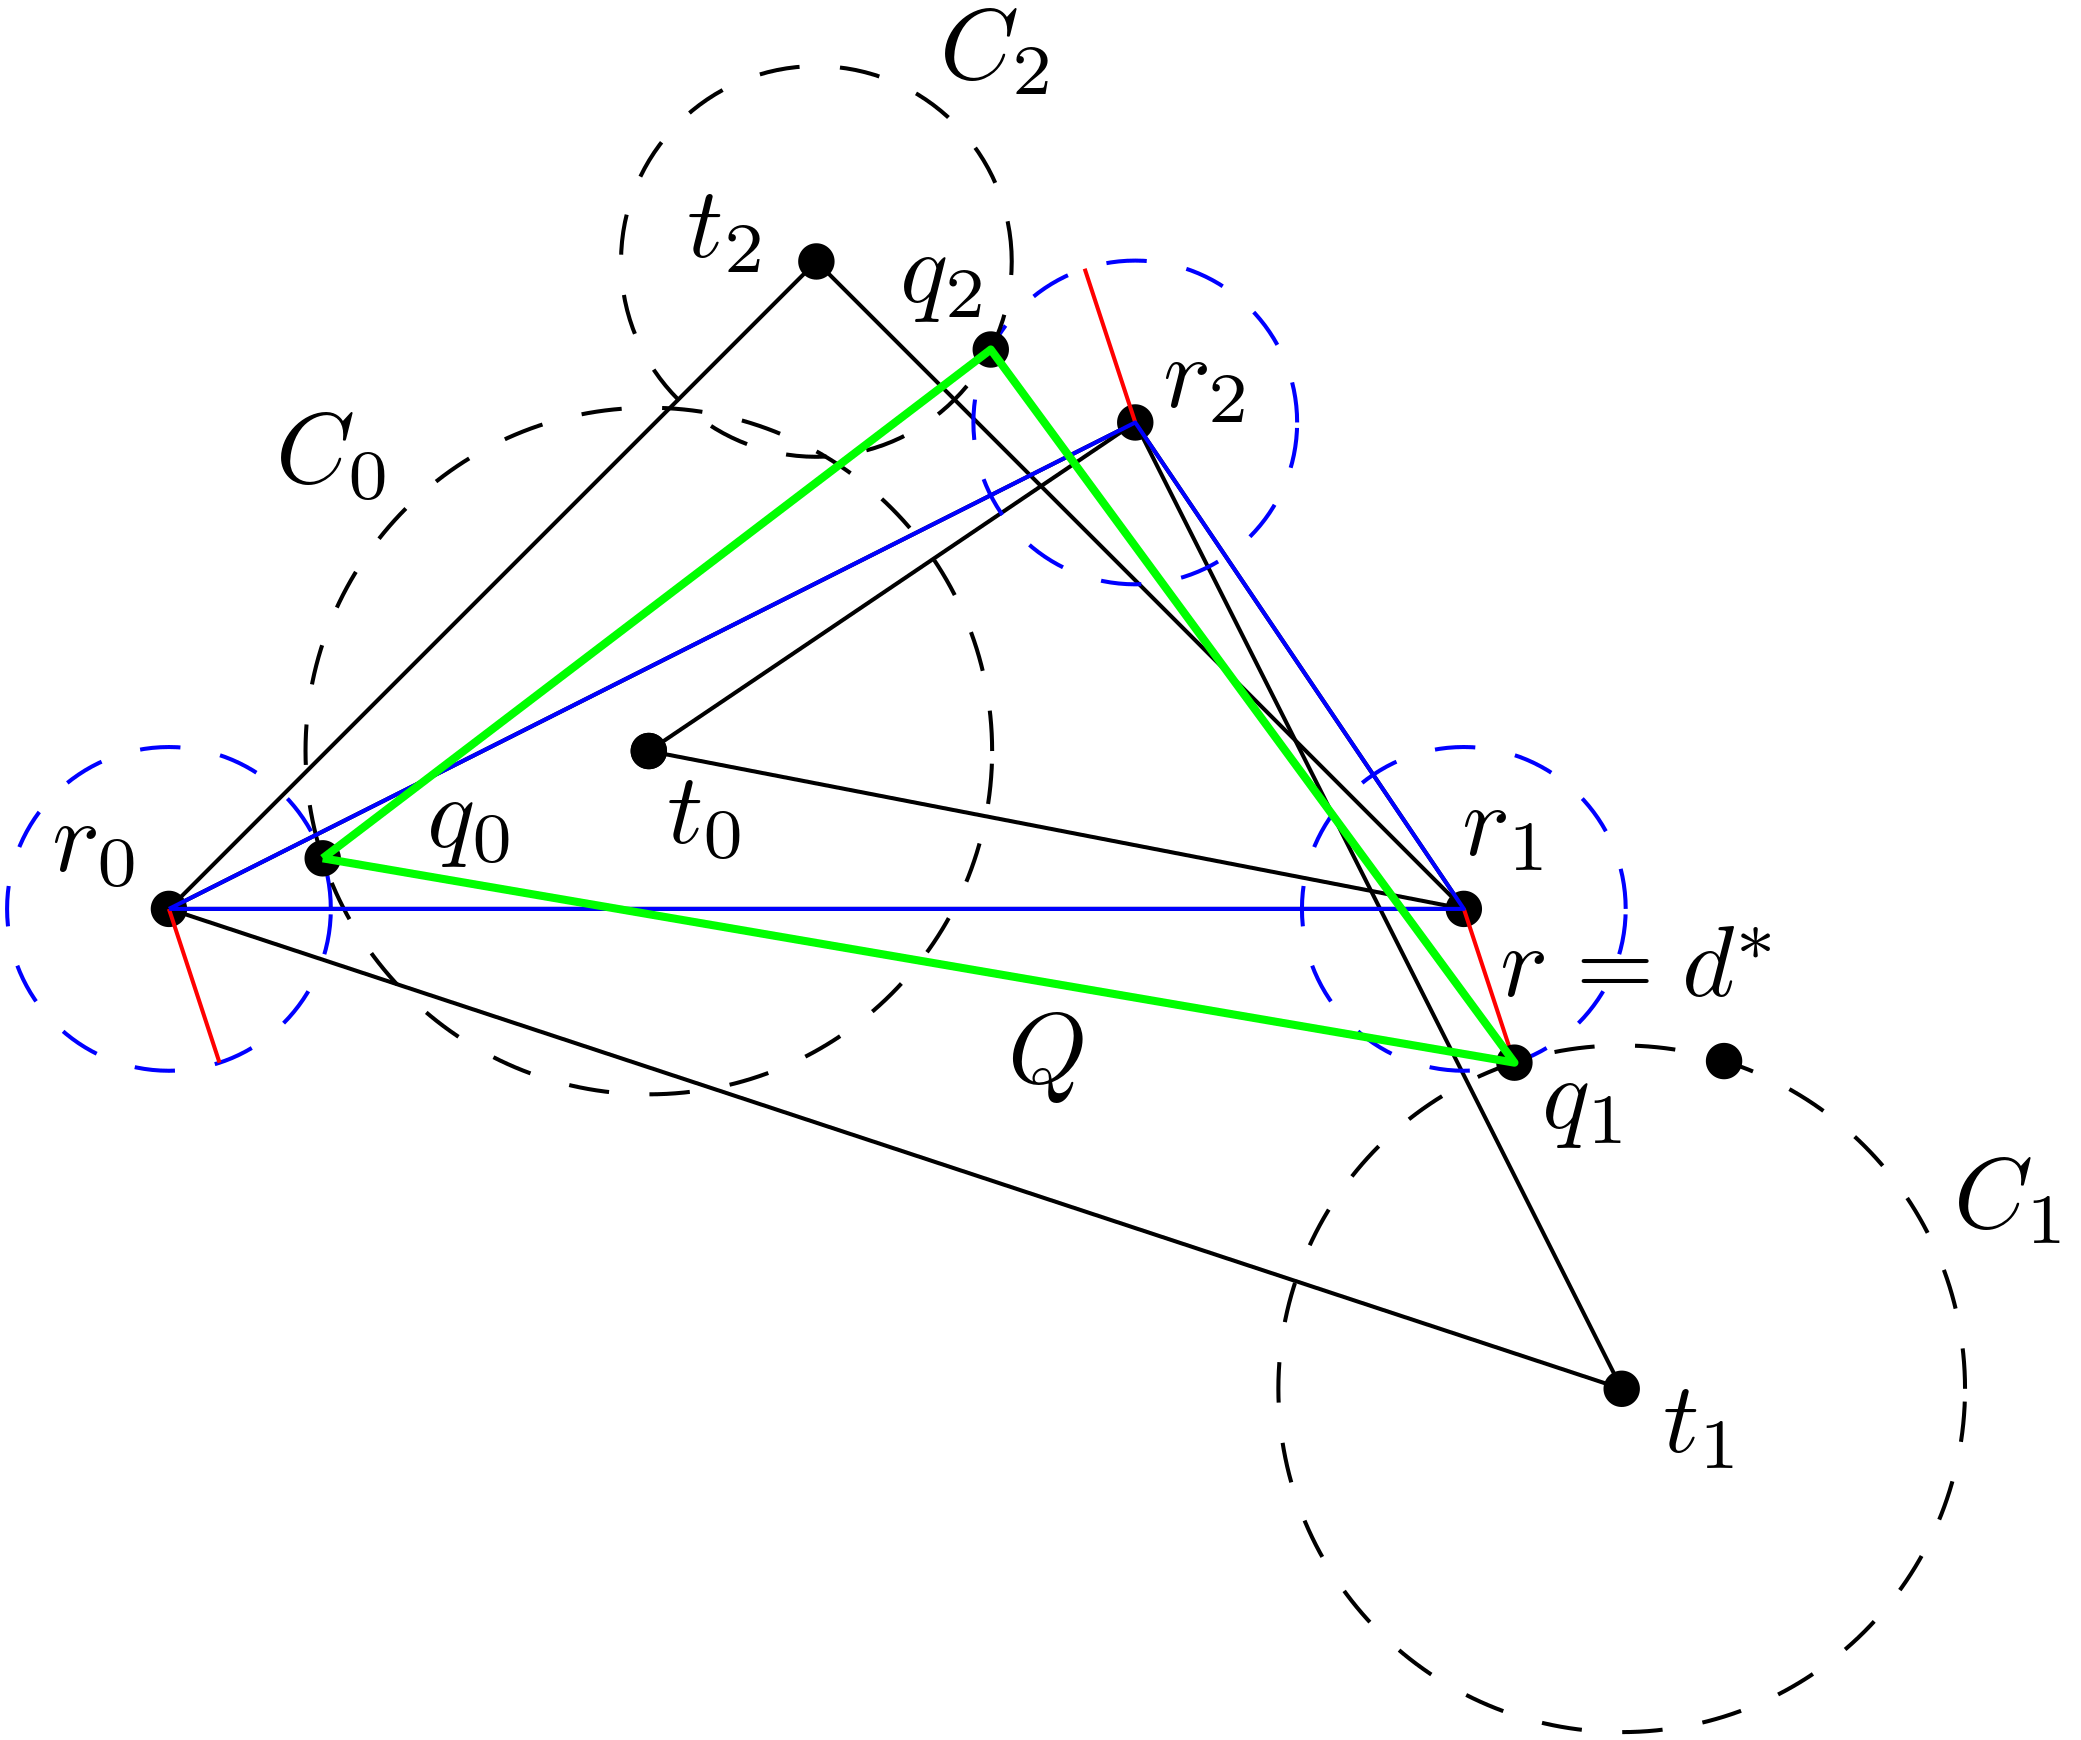
\includegraphics[width=\textwidth]{../media/construction_optimal.png}
                \end{center}
            \end{column}
        \end{columns}

        \framebreak

        \begin{columns}
            \begin{column}{0.5\textwidth}
                \begin{proof}[\proofname\ (Cont.)]
                    Notice, that since $r^\prime < r$, then $C(p_i, r^\prime)$ and the $i^{th}$ circle generated by $\mathcal{S}$ do not intersect.
            
                    \bigskip
            
                    Therefore, there exists no $Q^\prime \in \mathcal{S}$ such that $q_i \in C(p_i, r^\prime)$.

                    \bigskip

                    This is a contradiction.
                \end{proof}
                
            \end{column}
            \begin{column}{0.5\textwidth}  %%<--- here
                \begin{center}
                    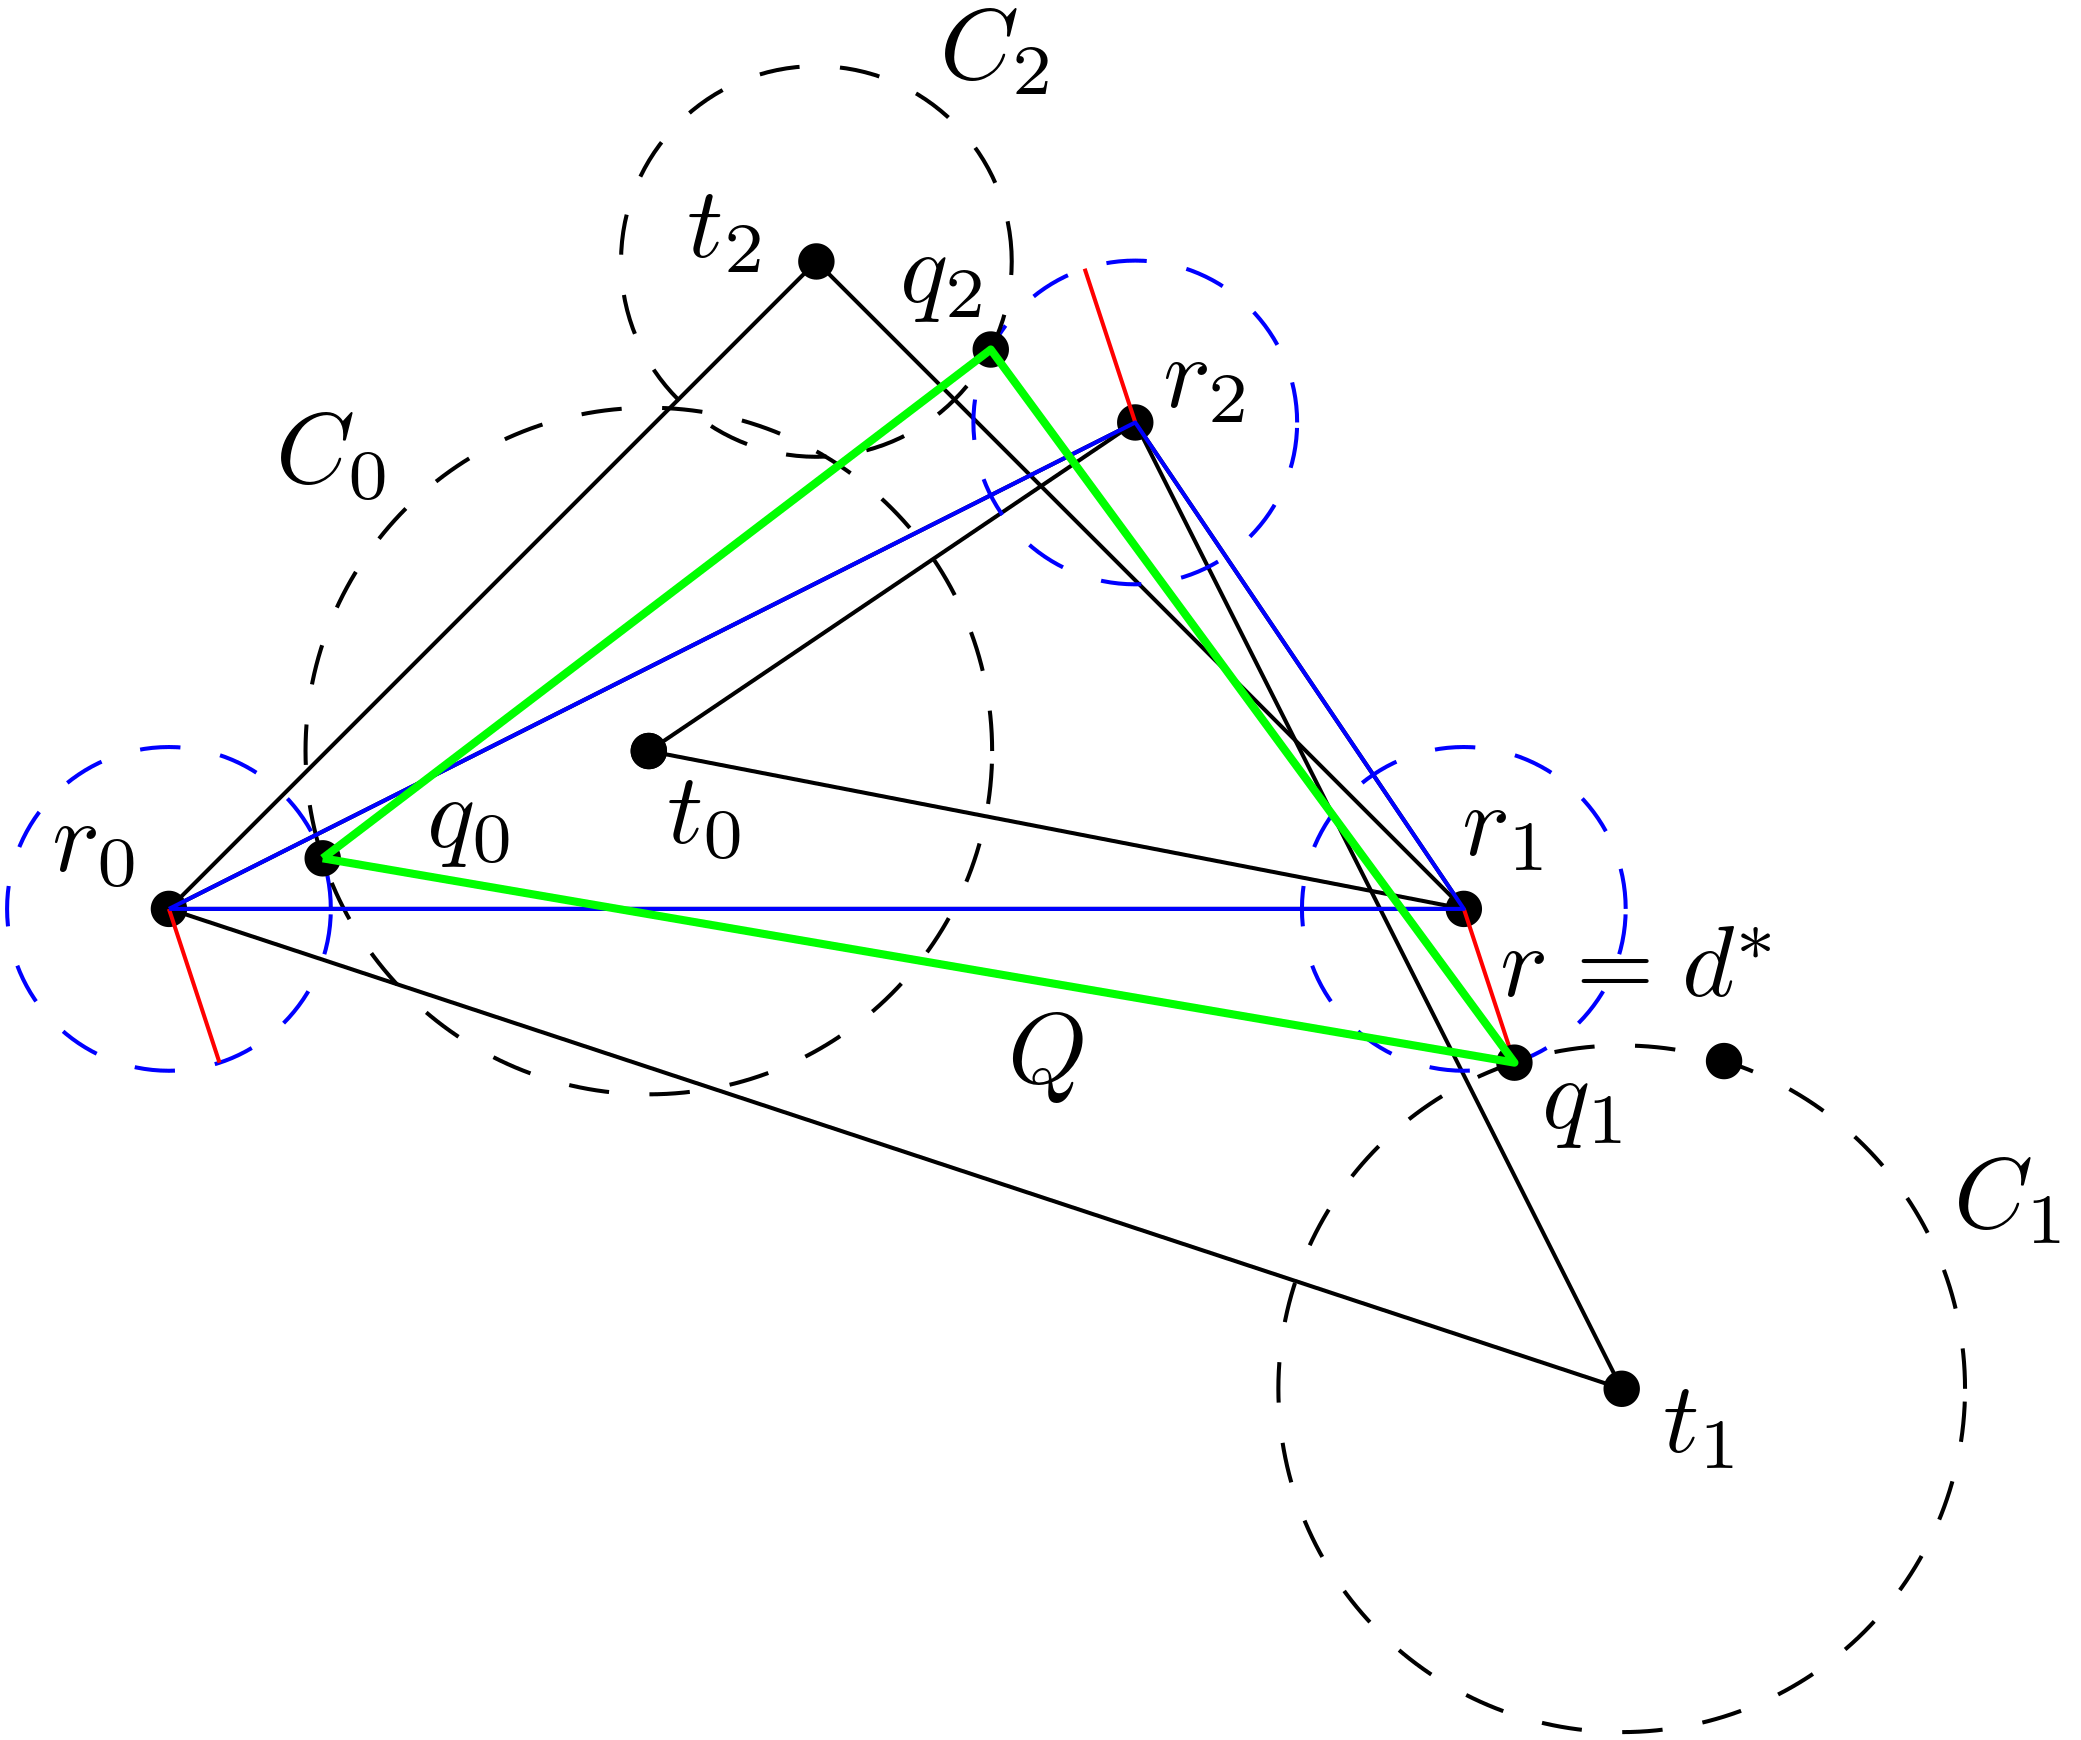
\includegraphics[width=\textwidth]{../media/construction_optimal.png}
                \end{center}
            \end{column}
        \end{columns}
    \end{frame}

    \begin{frame}{Assignment}
        \begin{itemize}
            \item Previous solution assumes a prescribed assignment between robots and their relative position in the pattern.
            \item Must test all possible assignments.
            \item Systems of three robots have $6$ possible assignments.
            \item Later, we introduce an optimization to avoid computing for all $6$ assignments.
        \end{itemize}    
    \end{frame}

    \begin{frame}{Observations}
        \framesubtitle{Focal Point}
        
        \begin{theorem}
            Given a set of three robots arbitrarily deployed on the plane at positions $P$, a pattern $S$, and the optimal solution, $Q^*$ there exists a single point that every robot moves either toward or away from.
        \end{theorem} 

    \end{frame}

    \begin{frame}[allowframebreaks]{Observations}
        \framesubtitle{Center-of-Mass Invariant}
        
        \begin{lemma}
            When $S$ forms an equilateral triangle, the center of mass of the original formation is the same as the destination formation.
            Furthermore, if every robot moves at the same speed, then the center of mass of all three robots never changes as they move toward their final destination in the formation. 
        \end{lemma}

        \framebreak

        \begin{columns}
            \begin{column}{0.5\textwidth}      
                \begin{proofs}
                    Note the center of mass is: 
                    $c = \left( \frac{r^x_0 + r^x_1 + r^x_2}{3}, \frac{r^y_0 + r^y_1 + r^y_2}{3}\right)$

                    \bigskip

                    Suppose $r_0$ and $r_1$ move towards the origin and $r_1$ moves away from the origin with a speed of $1$. 
                \end{proofs}
            \end{column}
            \begin{column}{0.5\textwidth}  %%<--- here
                \begin{center}
                    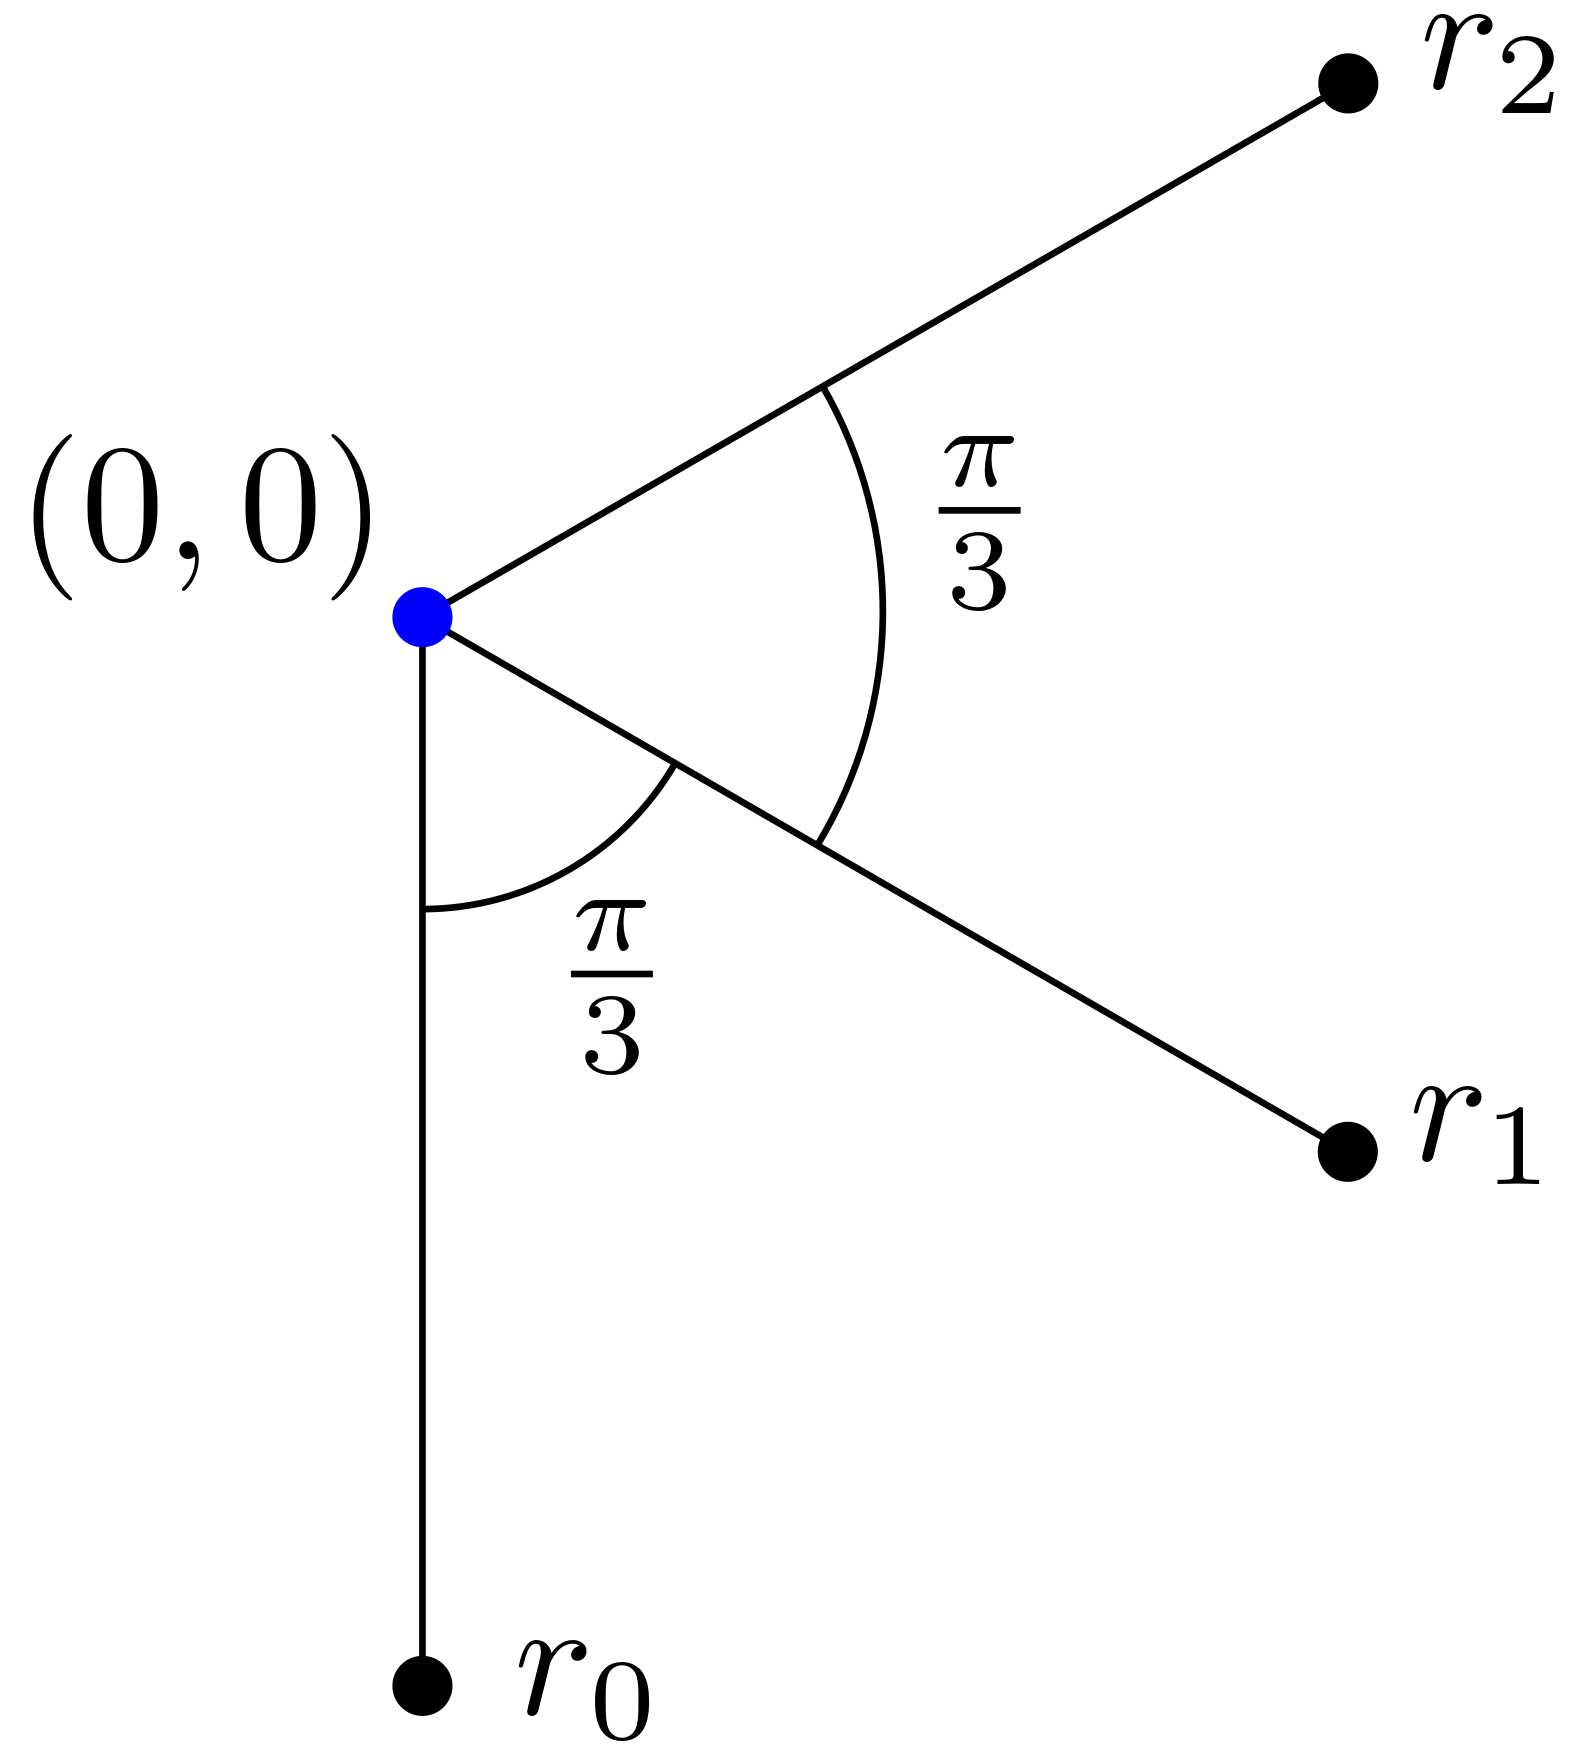
\includegraphics[width=\textwidth]{../media/center_of_mass.png}
                \end{center}
            \end{column}
        \end{columns}

        \framebreak

        \begin{columns}
            \begin{column}{0.6\textwidth}     
                \begin{proof}[\proofname\ (Cont.)]
                    
                    Then, after a single time step:
        
                    \begin{align*}
                        c^\prime &= \left( \frac{r^x_0 + (r^x_1 + cos \frac{\pi}{6}) + (r^x_2 - cos \frac{\pi}{6})}{3},\right. \\
                        &\quad \quad \left. \frac{(r^y_0 + 1) + (r^y_1 - sin \frac{\pi}{6}) + (r^y_2 - sin \frac{\pi}{6})}{3}\right) \\
                        &= \left( \frac{r^x_0 + r^x_1 + r^x_2}{3}, \frac{r^y_0 + r^y_1 + r^y_2}{3}\right) = c
                    \end{align*}
                \end{proof}
            \end{column}
            \begin{column}{0.4\textwidth}  %%<--- here
                \begin{center}
                    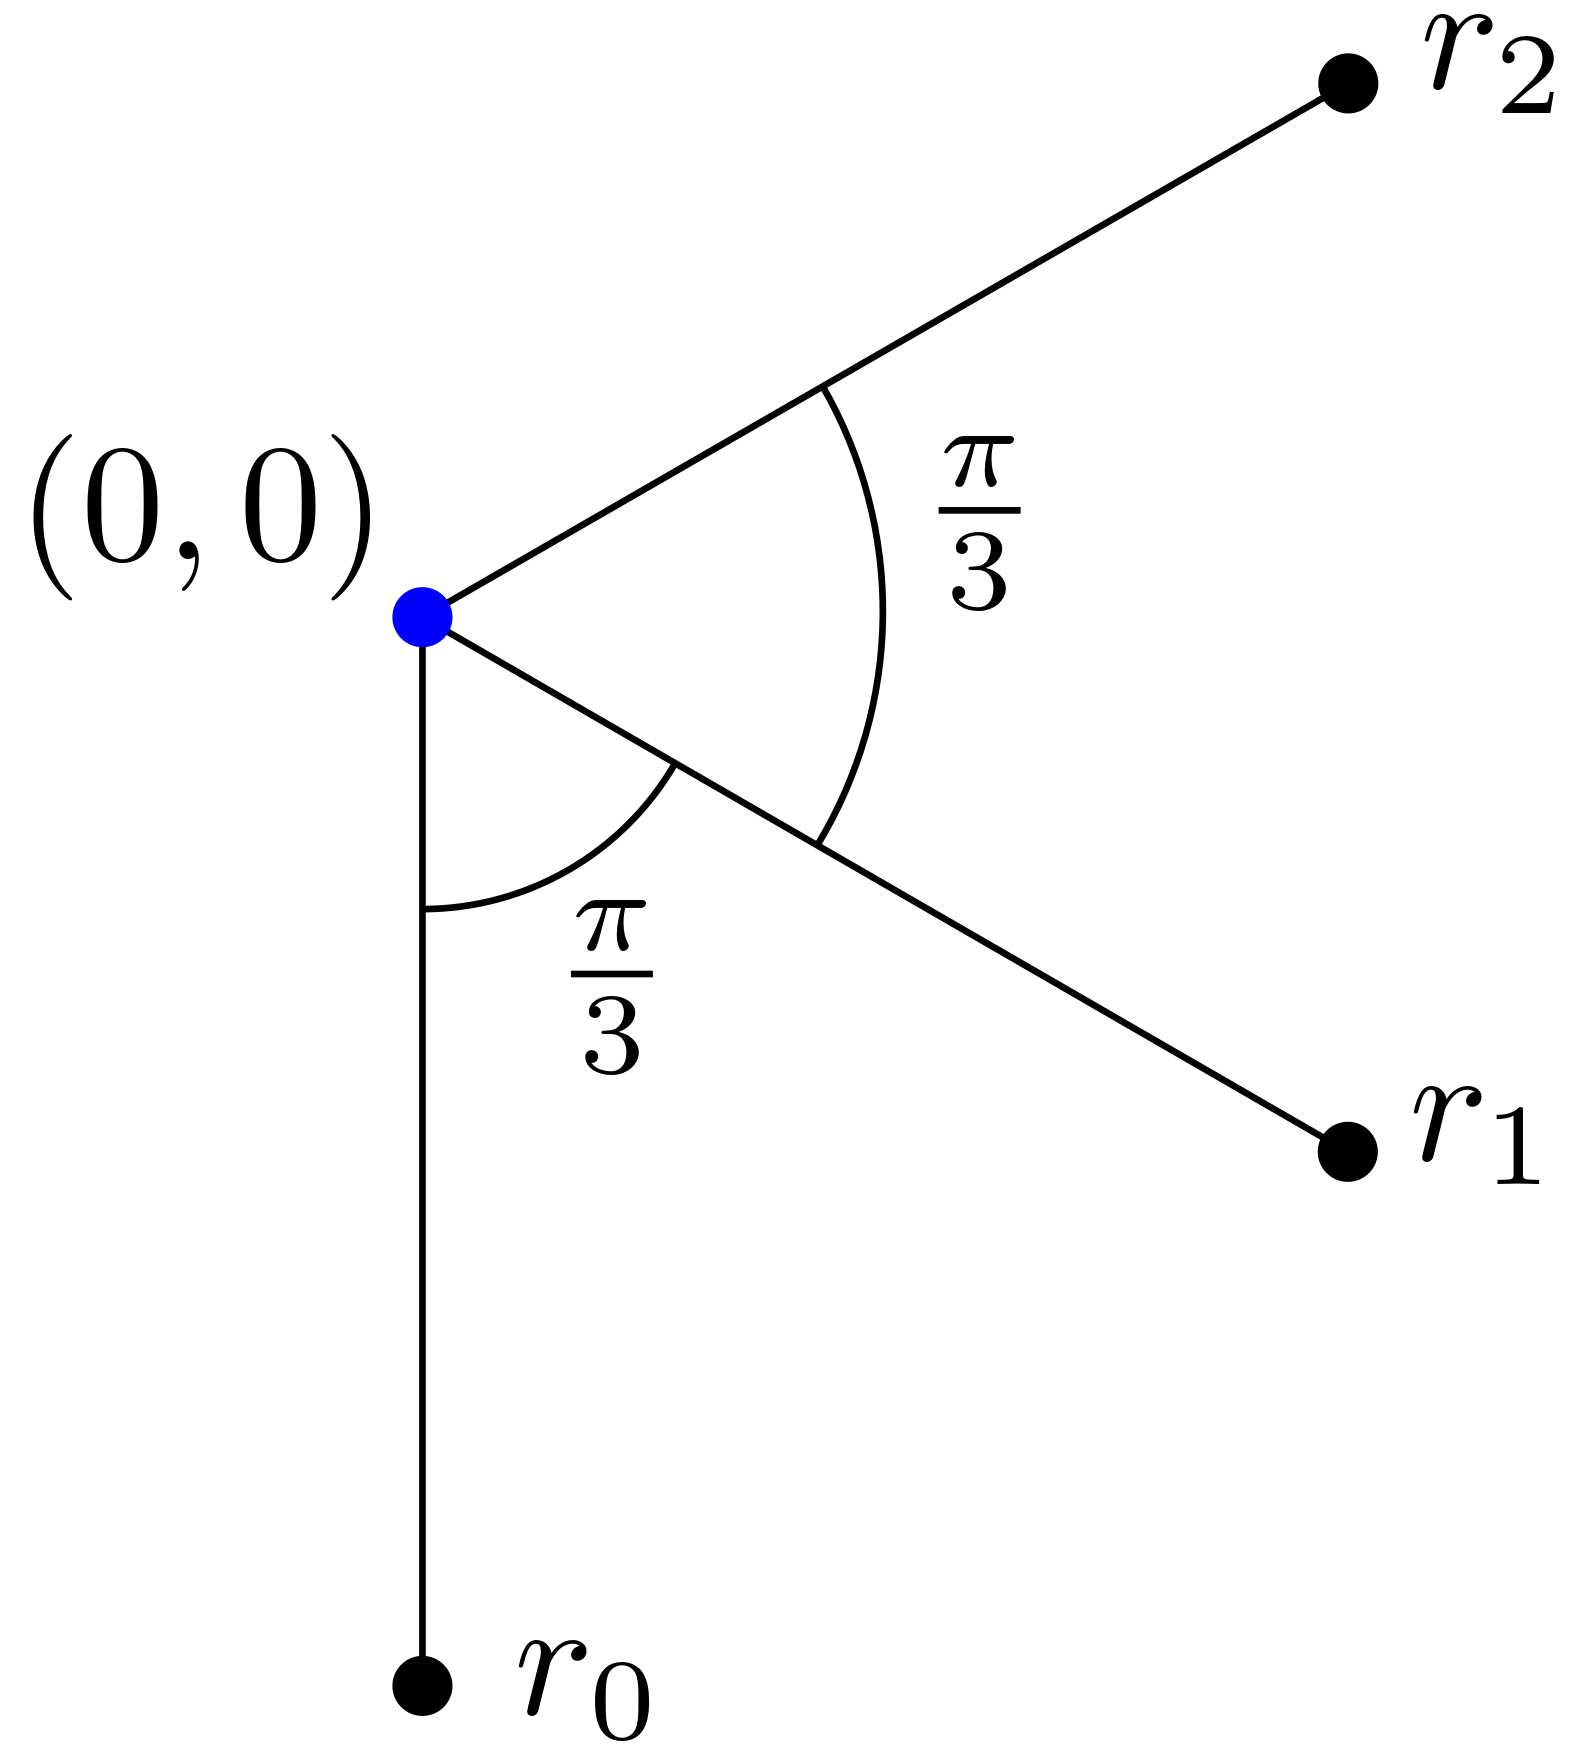
\includegraphics[width=0.7\textwidth]{../media/center_of_mass.png}
                \end{center}
            \end{column}
        \end{columns}
    \end{frame}

    \begin{frame}[allowframebreaks]{Observations}
        \framesubtitle{Invariance to Obliviousness}
        
        \begin{lemma}
            If all robots move at the same speed, any optimal solution is invariant with respect to time.
        \end{lemma}

        \framebreak

        \begin{proofs}
            Let $t^*$ be the time that every robot reaches its destination, or $f_i(t^*) = p_i$.
            
            Let $Q^{t}$ bethe optimal solution computed at time $t$.

            Suppose at time $t < t^*$, the robot has moved some distance 
            $r < d(p_i, q_i)$.

            Let $\hat{r}$ be the distance the robot has left to travel, should it continue towards $q_i$, or $\hat{r} = d(p_i, q_i) - r$.
        \end{proofs}

        \framebreak

        \begin{proof}[\proofname\ (Cont.)]
            First, note that 
            $d(p_i, q^{t}_i) \geq d(p_i, q_i)$, 
            or else $Q^*$ would not be optimal for the initial configuration. 
            
            Also, notice that
            $d(f_i(t), q^{t}_i) \leq d(f_i(t), q_i^*)$, or else
            $Q*$ is a better solution than $Q^{t}$, which is a contradiction to the assumption that $P^{t}$ is optimal.

            The only point where both of these conditions are satisfied is 
            $P^{t} = P^*$
        \end{proof}

        \framebreak

        \begin{center}
            \includemedia[
                width=0.7\textwidth,height=0.7\linewidth,
                activate=pageopen,
                transparent,
                addresource=../media/solution_set.mp4,
                flashvars={source=../media/solution_set.mp4&autoPlay=true&loop=true}
                ]{}{VPlayer.swf}
        \end{center}
    \end{frame}

    \begin{frame}[allowframebreaks]{Observations}
        \framesubtitle{Center Invariant}
        
        \begin{theorem}
            The center-of-mass of optimal solution is the incenter of circumcenters of the trivial replications used to compute it.
        \end{theorem} 
    \end{frame}

    \section{The General Case}

    \begin{frame}{The General Case}
        \framesubtitle{A Partial Solution}
        
        \begin{itemize}
            \item We know at least $3$ robots must move distance $d^*$
            \item There are $\binom{n}{3} \times \binom{n}{3} = \mathcal{O}(n^6)$ possible assignments where exactly $3$ robots move $d^*$.
            \item Thus, in the case where exactly $3$ robots move distance $d^*$, a solution can be found in $\mathcal{O}(n^8)$.
            \begin{itemize}
                \item Using an $\mathcal{O}(n^2)$ min-max maximum cardinality matching for each possible assignment.
            \end{itemize}
        \end{itemize}
    
    \end{frame}

\end{document}
